% --- LaTeX Lecture Notes Template - S. Venkatraman ---

% --- Set document class and font size ---

\documentclass[10pt,letterpaper]{article}


% --- Package imports ---

% Extended set of colors
\usepackage[dvipsnames]{xcolor}

\usepackage{
  amsmath, amsthm, amssymb, mathtools, dsfont, units,          % Math typesetting
  graphicx, wrapfig, subfig, float,                            % Figures and graphics formatting
  listings, color, inconsolata, pythonhighlight,               % Code formatting
  fancyhdr, sectsty, hyperref, enumerate, enumitem, framed }   % Headers/footers, section fonts, links, lists

% lipsum is just for generating placeholder text and can be removed
\usepackage{hyperref, lipsum} 
% \usepackage{bm}
% \usepackage{subfig}

% --- Fonts ---

\usepackage{newpxtext, newpxmath, inconsolata}
\usepackage{amsfonts}
\usepackage{pgfplots}
\pgfplotsset{compat=1.12}
\usepackage{tkz-fct}
\usepackage{svg}
\usepackage{tikz}
\usepackage{tikz-cd}
\usepackage{lipsum}
\usepackage{enumitem}
\usepackage[title]{appendix}
% \usepackage[toc,page]{appxendix}
\usepackage[utf8]{inputenc}
\usepackage{multicol}
\usepackage{multirow}
\usepackage{booktabs}

\usepackage{minted}  % code highlighting
% \usepackage[finalizecache,cachedir=.]{minted}
% \usepackage[frozencache,cachedir=.]{minted}

\DeclareUnicodeCharacter{3BC}{$\pi$}
\DeclareUnicodeCharacter{3C0}{$\pi$}

\usepackage[most]{tcolorbox}
\newtcolorbox{myquote}[1][]{%
  colback=black!5,
  colframe=black!5,
  notitle,
  sharp corners,
  % borderline west={2pt}{0pt}{red!80!black},
  enhanced,
  breakable,
}

\renewcommand*\pod[1]{%
  \allowbreak
  \mathchoice
    {\mkern 18mu}%
    {\mkern  8mu}%
    {\mkern  6mu}% "6mu" matches the space *after* the word "mod"
    {\mkern  6mu}%
  (#1)%
}

% --- Page layout settings ---

% Set page margins
\usepackage[left=1.35in, right=1.35in, top=1.0in, bottom=.9in, headsep=.2in, footskip=0.35in]{geometry}

% Anchor footnotes to the bottom of the page
\usepackage[bottom]{footmisc}

% Set line spacing
\renewcommand{\baselinestretch}{1.2}

% Set spacing between paragraphs
\setlength{\parskip}{1.3mm}

% Allow multi-line equations to break onto the next page
\allowdisplaybreaks

% --- Page formatting settings ---

% Set image captions to be italicized
\usepackage[font={it,footnotesize}]{caption}

% Set link colors for labeled items (blue), citations (red), URLs (orange)
\hypersetup{colorlinks=true, linkcolor=RoyalBlue, citecolor=RedOrange, urlcolor=ForestGreen}

% Set font size for section titles (\large) and subtitles (\normalsize) 
\usepackage{titlesec}
% \titleformat{\section}{\large\bfseries}{{\fontsize{19}{19}\selectfont\textreferencemark}\;\; }{0em}{}
\titleformat{\section}{\large\bfseries}{\thesection\;\;\;}{0em}{}
\titleformat{\subsection}{\normalsize\bfseries\selectfont}{\thesubsection\;\;\;}{0em}{}

% Enumerated/bulleted lists: make numbers/bullets flush left
%\setlist[enumerate]{wide=2pt, leftmargin=16pt, labelwidth=0pt}
\setlist[itemize]{wide=0pt, leftmargin=16pt, labelwidth=10pt, align=left}

% --- Table of contents settings ---

\usepackage[subfigure]{tocloft}

% Reduce spacing between sections in table of contents
\setlength{\cftbeforesecskip}{.9ex}

% Remove indentation for sections
\cftsetindents{section}{0em}{0em}

% Set font size (\large) for table of contents title
\renewcommand{\cfttoctitlefont}{\large\bfseries}

% Remove numbers/bullets from section titles in table of contents
\makeatletter
\renewcommand{\cftsecpresnum}{\begin{lrbox}{\@tempboxa}}
\renewcommand{\cftsecaftersnum}{\end{lrbox}}
\makeatother

% --- Set path for images ---

\graphicspath{{Images/}{../Images/}}

% --- Math/Statistics commands ---

% Add a reference number to a single line of a multi-line equation
% Usage: "\numberthis\label{labelNameHere}" in an align or gather environment
\newcommand\numberthis{\addtocounter{equation}{1}\tag{\theequation}}

% Shortcut for bold text in math mode, e.g. $\b{X}$
\let\b\mathbf

% Shortcut for bold Greek letters, e.g. $\bg{\beta}$
\let\bg\boldsymbol

% Shortcut for calligraphic script, e.g. %\mc{M}$
\let\mc\mathcal

% \mathscr{(letter here)} is sometimes used to denote vector spaces
\usepackage[mathscr]{euscript}

% Convergence: right arrow with optional text on top
% E.g. $\converge[p]$ for converges in probability
\newcommand{\converge}[1][]{\xrightarrow{#1}}

% Weak convergence: harpoon symbol with optional text on top
% E.g. $\wconverge[n\to\infty]$
\newcommand{\wconverge}[1][]{\stackrel{#1}{\rightharpoonup}}

% Equality: equals sign with optional text on top
% E.g. $X \equals[d] Y$ for equality in distribution
\newcommand{\equals}[1][]{\stackrel{\smash{#1}}{=}}

% Normal distribution: arguments are the mean and variance
% E.g. $\normal{\mu}{\sigma}$
\newcommand{\normal}[2]{\mathcal{N}\left(#1,#2\right)}

% Uniform distribution: arguments are the left and right endpoints
% E.g. $\unif{0}{1}$
\newcommand{\unif}[2]{\text{Uniform}(#1,#2)}

% Independent and identically distributed random variables
% E.g. $ X_1,...,X_n \iid \normal{0}{1}$
\newcommand{\iid}{\stackrel{\smash{\text{iid}}}{\sim}}

% Sequences (this shortcut is mostly to reduce finger strain for small hands)
% E.g. to write $\{A_n\}_{n\geq 1}$, do $\bk{A_n}{n\geq 1}$
\newcommand{\bk}[2]{\{#1\}_{#2}}

\newcommand{\what}[1]{\widehat{#1}}
% \setcounter{section}{-1}

\setcounter{MaxMatrixCols}{20}

\newcommand{\SL}{\mathrm{SL}}
\newcommand{\Sp}{\mathrm{Sp}}
\newcommand{\Mp}{\mathrm{Mp}}
\newcommand{\GL}{\mathrm{GL}}
\newcommand{\SO}{\mathrm{SO}}
\newcommand{\SU}{\mathrm{SU}}
\newcommand{\PGL}{\mathrm{PGL}}
\newcommand{\PSL}{\mathrm{PSL}}
\newcommand{\GSp}{\mathrm{GSp}}
\newcommand{\PGSp}{\mathrm{PGSp}}
\newcommand{\Spin}{\mathrm{Spin}}
\newcommand{\gl}{\mathfrak{gl}}
\newcommand{\JL}{\mathrm{JL}}
\newcommand{\stab}{\mathrm{Stab}}
% \newcommand{\ab}{\mathrm{ab}}
\newcommand{\cha}{\mathrm{char}}
\newcommand{\fin}{\mathrm{fin}}
\newcommand{\Tr}{\mathrm{Tr}}
\newcommand{\Li}{\mathrm{Li}}
\newcommand{\trdeg}{\mathrm{trdeg}}
\newcommand{\rank}{\mathrm{rank}}
\newcommand{\rad}{\mathrm{rad}}
\newcommand{\Res}{\mathrm{Res}}
\newcommand{\Hom}{\mathrm{Hom}}
\newcommand{\Spec}{\mathrm{Spec}\,}
\newcommand{\Sym}{\mathrm{Sym}}
\newcommand{\ev}{\mathrm{ev}}
\newcommand{\disc}{\mathrm{disc}}
\newcommand{\Aut}{\mathrm{Aut}}
\newcommand{\Span}{\mathrm{Span}}
\newcommand{\supp}{\mathrm{supp}}
\newcommand{\sgn}{\mathrm{sgn}}
\newcommand{\Lie}{\mathrm{Lie}}
\newcommand{\Ind}{\mathrm{Ind}}
\newcommand{\pInd}{\mathrm{pInd}}
\newcommand{\Gal}{\mathrm{Gal}}
\newcommand{\Cl}{\mathrm{Cl}}
\newcommand{\Wh}{\mathrm{Wh}}
\newcommand{\std}{\mathrm{std}}
\newcommand{\Slit}{\mathrm{Slit}}
\newcommand{\pprod}{\sideset{}{'}\prod}
\newcommand{\potimes}{\sideset{}{'}\otimes}
\newcommand{\pbigotimes}{\sideset{}{'}\bigotimes}
% \sideset{}{'}\prod
\newcommand{\RQM}{\mathcal{RQM}}

\newcommand{\QM}{\mathcal{QM}}

\newcommand{\dd}{\mathrm{d}}
\newcommand{\dso}{\mathds{1}}

\newcommand{\llb}{\llbracket}
\newcommand{\rrb}{\rrbracket}

\newcommand{\rA}{\mathrm{A}}
\newcommand{\rB}{\mathrm{B}}
\newcommand{\rC}{\mathrm{C}}
\newcommand{\rD}{\mathrm{D}}
\newcommand{\rE}{\mathrm{E}}
\newcommand{\rF}{\mathrm{F}}
\newcommand{\rG}{\mathrm{G}}
\newcommand{\rH}{\mathrm{H}}
\newcommand{\rI}{\mathrm{I}}
\newcommand{\rJ}{\mathrm{J}}
\newcommand{\rK}{\mathrm{K}}
\newcommand{\rL}{\mathrm{L}}
\newcommand{\rM}{\mathrm{M}}
\newcommand{\rN}{\mathrm{N}}
\newcommand{\rO}{\mathrm{O}}
\newcommand{\rP}{\mathrm{P}}
\newcommand{\rQ}{\mathrm{Q}}
\newcommand{\rR}{\mathrm{R}}
\newcommand{\rS}{\mathrm{S}}
\newcommand{\rT}{\mathrm{T}}
\newcommand{\rU}{\mathrm{U}}
\newcommand{\rV}{\mathrm{V}}
\newcommand{\rW}{\mathrm{W}}
\newcommand{\rX}{\mathrm{X}}
\newcommand{\rY}{\mathrm{Y}}
\newcommand{\rZ}{\mathrm{Z}}

\newcommand{\bA}{\mathbb{A}}
\newcommand{\bB}{\mathbb{B}}
\newcommand{\bC}{\mathbb{C}}
\newcommand{\bD}{\mathbb{D}}
\newcommand{\bE}{\mathbb{E}}
\newcommand{\bF}{\mathbb{F}}
\newcommand{\bG}{\mathbb{G}}
\newcommand{\bH}{\mathbb{H}}
\newcommand{\bI}{\mathbb{I}}
\newcommand{\bJ}{\mathbb{J}}
\newcommand{\bK}{\mathbb{K}}
\newcommand{\bL}{\mathbb{L}}
\newcommand{\bM}{\mathbb{M}}
\newcommand{\bN}{\mathbb{N}}
\newcommand{\bO}{\mathbb{O}}
\newcommand{\bP}{\mathbb{P}}
\newcommand{\bQ}{\mathbb{Q}}
\newcommand{\bR}{\mathbb{R}}
\newcommand{\bS}{\mathbb{S}}
\newcommand{\bT}{\mathbb{T}}
\newcommand{\bU}{\mathbb{U}}
\newcommand{\bV}{\mathbb{V}}
\newcommand{\bW}{\mathbb{W}}
\newcommand{\bX}{\mathbb{X}}
\newcommand{\bY}{\mathbb{Y}}
\newcommand{\bZ}{\mathbb{Z}}

\newcommand{\bx}{\mathbf{x}}
\newcommand{\by}{\mathbf{y}}

\newcommand{\cA}{\mathcal{A}}
\newcommand{\cB}{\mathcal{B}}
\newcommand{\cC}{\mathcal{C}}
\newcommand{\cD}{\mathcal{D}}
\newcommand{\cE}{\mathcal{E}}
\newcommand{\cF}{\mathcal{F}}
\newcommand{\cG}{\mathcal{G}}
\newcommand{\cH}{\mathcal{H}}
\newcommand{\cI}{\mathcal{I}}
\newcommand{\cJ}{\mathcal{J}}
\newcommand{\cK}{\mathcal{K}}
\newcommand{\cL}{\mathcal{L}}
\newcommand{\cM}{\mathcal{M}}
\newcommand{\cN}{\mathcal{N}}
\newcommand{\cO}{\mathcal{O}}
\newcommand{\cP}{\mathcal{P}}
\newcommand{\cQ}{\mathcal{Q}}
\newcommand{\cR}{\mathcal{R}}
\newcommand{\cS}{\mathcal{S}}
\newcommand{\cT}{\mathcal{T}}
\newcommand{\cU}{\mathcal{U}}
\newcommand{\cV}{\mathcal{V}}
\newcommand{\cW}{\mathcal{W}}
\newcommand{\cX}{\mathcal{X}}
\newcommand{\cY}{\mathcal{Y}}
\newcommand{\cZ}{\mathcal{Z}}

\newcommand{\scA}{\mathscr{A}}
\newcommand{\scB}{\mathscr{B}}
\newcommand{\scC}{\mathscr{C}}
\newcommand{\scD}{\mathscr{D}}
\newcommand{\scE}{\mathscr{E}}
\newcommand{\scF}{\mathscr{F}}
\newcommand{\scG}{\mathscr{G}}
\newcommand{\scH}{\mathscr{H}}
\newcommand{\scI}{\mathscr{I}}
\newcommand{\scJ}{\mathscr{J}}
\newcommand{\scK}{\mathscr{K}}
\newcommand{\scL}{\mathscr{L}}
\newcommand{\scM}{\mathscr{M}}
\newcommand{\scN}{\mathscr{N}}
\newcommand{\scO}{\mathscr{O}}
\newcommand{\scP}{\mathscr{P}}
\newcommand{\scQ}{\mathscr{Q}}
\newcommand{\scR}{\mathscr{R}}
\newcommand{\scS}{\mathscr{S}}
\newcommand{\scT}{\mathscr{T}}
\newcommand{\scU}{\mathscr{U}}
\newcommand{\scV}{\mathscr{V}}
\newcommand{\scW}{\mathscr{W}}
\newcommand{\scX}{\mathscr{X}}
\newcommand{\scY}{\mathscr{Y}}
\newcommand{\scZ}{\mathscr{Z}}

\newcommand{\frA}{\mathfrak{A}}
\newcommand{\frB}{\mathfrak{B}}
\newcommand{\frC}{\mathfrak{C}}
\newcommand{\frD}{\mathfrak{D}}
\newcommand{\frE}{\mathfrak{E}}
\newcommand{\frF}{\mathfrak{F}}
\newcommand{\frG}{\mathfrak{G}}
\newcommand{\frH}{\mathfrak{H}}
\newcommand{\frI}{\mathfrak{I}}
\newcommand{\frJ}{\mathfrak{J}}
\newcommand{\frK}{\mathfrak{K}}
\newcommand{\frL}{\mathfrak{L}}
\newcommand{\frM}{\mathfrak{M}}
\newcommand{\frN}{\mathfrak{N}}
\newcommand{\frO}{\mathfrak{O}}
\newcommand{\frP}{\mathfrak{P}}
\newcommand{\frQ}{\mathfrak{Q}}
\newcommand{\frR}{\mathfrak{R}}
\newcommand{\frS}{\mathfrak{S}}
\newcommand{\frT}{\mathfrak{T}}
\newcommand{\frU}{\mathfrak{U}}
\newcommand{\frV}{\mathfrak{V}}
\newcommand{\frW}{\mathfrak{W}}
\newcommand{\frX}{\mathfrak{X}}
\newcommand{\frY}{\mathfrak{Y}}
\newcommand{\frZ}{\mathfrak{Z}}

\newcommand{\fra}{\mathfrak{a}}
\newcommand{\frb}{\mathfrak{b}}
\newcommand{\frc}{\mathfrak{c}}
\newcommand{\frd}{\mathfrak{d}}
\newcommand{\fre}{\mathfrak{e}}
\newcommand{\frf}{\mathfrak{f}}
\newcommand{\frg}{\mathfrak{g}}
\newcommand{\frh}{\mathfrak{h}}
\newcommand{\fri}{\mathfrak{i}}
\newcommand{\frj}{\mathfrak{j}}
\newcommand{\frk}{\mathfrak{k}}
\newcommand{\frl}{\mathfrak{l}}
\newcommand{\frm}{\mathfrak{m}}
\newcommand{\frn}{\mathfrak{n}}
\newcommand{\fro}{\mathfrak{o}}
\newcommand{\frp}{\mathfrak{p}}
\newcommand{\frq}{\mathfrak{q}}
\newcommand{\frr}{\mathfrak{r}}
\newcommand{\frs}{\mathfrak{s}}
\newcommand{\frt}{\mathfrak{t}}
\newcommand{\fru}{\mathfrak{u}}
\newcommand{\frv}{\mathfrak{v}}
\newcommand{\frw}{\mathfrak{w}}
\newcommand{\frx}{\mathfrak{x}}
\newcommand{\fry}{\mathfrak{y}}
\newcommand{\frz}{\mathfrak{z}}

\newcommand{\sage}{\raisebox{-0.16\height}{
\includegraphics[height=1em]{./sagelogo.png}}\,\,}

% Math mode symbols for common sets and spaces. Example usage: $\R$
\newcommand{\R}{\mathbb{R}}	% Real numbers
\newcommand{\C}{\mathbb{C}}	% Complex numbers
\newcommand{\Q}{\mathbb{Q}}	% Rational numbers
\newcommand{\Z}{\mathbb{Z}}	% Integers
\newcommand{\N}{\mathbb{N}}	% Natural numbers
\newcommand{\F}{\mathcal{F}}	% Calligraphic F for a sigma algebra
\newcommand{\El}{\mathcal{L}}	% Calligraphic L, e.g. for L^p spaces

% Math mode symbols for probability
\newcommand{\pr}{\mathbb{P}}	% Probability measure
\newcommand{\E}{\mathbb{E}}	% Expectation, e.g. $\E(X)$
\newcommand{\var}{\text{Var}}	% Variance, e.g. $\var(X)$
\newcommand{\cov}{\text{Cov}}	% Covariance, e.g. $\cov(X,Y)$
\newcommand{\corr}{\text{Corr}}	% Correlation, e.g. $\corr(X,Y)$
\newcommand{\B}{\mathcal{B}}	% Borel sigma-algebra

% Other miscellaneous symbols
\newcommand{\tth}{\text{th}}	% Non-italicized 'th', e.g. $n^\tth$
\newcommand{\Oh}{\mathcal{O}}	% Big-O notation, e.g. $\O(n)$
\newcommand{\1}{\mathds{1}}	% Indicator function, e.g. $\1_A$

\newcommand{\nul}{\mathrm{null}}
\newcommand{\range}{\mathrm{range}}

% Additional commands for math mode
\newcommand*{\argmax}{argmax}		% Argmax, e.g. $\argmax_{x\in[0,1]} f(x)$
\newcommand*{\argmin}{argmin}		% Argmin, e.g. $\argmin_{x\in[0,1]} f(x)$
\newcommand*{\spann}{Span}		% Span, e.g. $\spann\{X_1,...,X_n\}$
\newcommand*{\bias}{Bias}		% Bias, e.g. $\bias(\hat\theta)$
\newcommand*{\ran}{ran}			% Range of an operator, e.g. $\ran(T) 
\newcommand*{\dv}{d\!}			% Non-italicized 'with respect to', e.g. $\int f(x) \dv x$
\newcommand*{\diag}{diag}		% Diagonal of a matrix, e.g. $\diag(M)$
\newcommand*{\trace}{Tr}		% Trace of a matrix, e.g. $\trace(M)$
% \newcommand*{\supp}{supp}		% Support of a function, e.g., $\supp(f)$

% Numbered theorem, lemma, etc. settings - e.g., a definition, lemma, and theorem appearing in that 
% order in Lecture 2 will be numbered Definition 2.1, Lemma 2.2, Theorem 2.3. 
% Example usage: \begin{theorem}[Name of theorem] Theorem statement \end{theorem}
\theoremstyle{definition}
\newtheorem{theorem}{Theorem}[section]
\newtheorem{proposition}[theorem]{Proposition}
\newtheorem{lemma}[theorem]{Lemma}
\newtheorem{corollary}[theorem]{Corollary}
\newtheorem{definition}[theorem]{Definition}
\newtheorem{example}[theorem]{Example}
\newtheorem{question}[theorem]{Question}
\newtheorem{conjecture}[theorem]{Conjecture}
\newtheorem{exercise}[subsubsection]{Exercise}

\theoremstyle{remark}
\newtheorem{remark}[theorem]{Remark}

% Un-numbered theorem, lemma, etc. settings
% Example usage: \begin{lemma*}[Name of lemma] Lemma statement \end{lemma*}
\newtheorem*{theorem*}{Theorem}
\newtheorem*{proposition*}{Proposition}
\newtheorem*{lemma*}{Lemma}
\newtheorem*{corollary*}{Corollary}
\newtheorem*{definition*}{Definition}
\newtheorem*{example*}{Example}
\newtheorem*{remark*}{Remark}
\newtheorem*{claim}{Claim}
\newtheorem*{conjecture*}{Conjecture}

% --- Left/right header text (to appear on every page) ---

% Do not include a line under header or above footer
\pagestyle{fancy}
\renewcommand{\footrulewidth}{0pt}
\renewcommand{\headrulewidth}{0pt}

% Right header text: Lecture number and title
\renewcommand{\sectionmark}[1]{\markright{#1} }
% \fancyhead[R]{\small\textit{\nouppercase{\rightmark}}}

% Left header text: Short course title, hyperlinked to table of contents
% \fancyhead[L]{\hyperref[sec:contents]{\small Matrix multplication}}

% \pgfkeys{/Dynkin diagram,
% edge length=1.5cm,
% fold radius=1cm,
% indefinite edge/.style={
% draw=black,
% fill=white,
% thin,
% densely dashed}}

\usepackage{fancyhdr}
\pagestyle{fancy}
\fancyhead[R]{}
\fancyhead[L]{}

% --- Document starts here ---

\begin{document}

% --- Main title and subtitle ---

\title{How automorphic forms and elliptic curves fly?}
% \\[1em]
% \normalsize Re-typed by Seewoo Lee\footnote{seewoo5@berkeley.edu}}

% --- Author and date of last update ---

\author{Seewoo Lee}
\date{\normalsize\vspace{-1ex} Last updated: \today}
% \date{}

% --- Add title and table of contents ---

\maketitle

% --- Abstracts ---

% \tableofcontents\label{sec:contents}
\begin{abstract}
    This is an expository note on \emph{murmurations}, which was initially discovered by He, Lee, Oliver, and Pozdnyakov for elliptic curves.
    We focus on the cases where the mumuration density is computed (under GRH), including the work of Zubrilina, Lee--Oliver--Pozdnyakov, and Sawin--Sutherland.
\end{abstract}

% --- Main content: import lectures as subfiles ---
\section{Introduction}
\label{sec:intro}

The goal of this note is to introduce the arithmetic of function fields, which is the analogue of number theory for polynomials.
Especially, our main goal is to study various evidences of the following claim:

\begin{myquote}
A theorem that holds for integers is also true for polynomials (over finite fields), and latter is often easier to prove.
\end{myquote}
For example, we will see a proof of Fermat's Last Theorem for polynomials, which only requires few pages to prove.

Dictionary between the integers and the polynomials over finite fields can be found in Table \ref{tab:dictionary} of Appendix.

\subsection*{Prerequisites}
We assume that the readers are familiar with undergraduate level algebra (groups, rings, fields, etc.), number theory (congruences, prime numbers, etc.), and a bit of complex analysis.
Some of the theory of finite fields will be reviewed in Appendix \ref{subsec:handbook_galois_ff}.


\subsection*{Notations}

Let $p$ be a prime number. We denote by $\bF_p$ the finite field of order $p$, which is the field with $p$ elements.
We denote the polynomial ring $\bF_p[T]$ by $A$.
For each nonzero polynomial $f \in A$, we denote it's norm by $|f| = p^{\deg (f)}$, where $\deg (f)$ is the degree of $f$, and we set $|0| = 0$.

\subsection*{Sage codes}

There are some codes in this note, which are mostly written in \href{https://www.sagemath.org/}{Sage}.
Sage is a free \href{https://github.com/sagemath/sage}{open-source} mathematics software system, which is built on top of many existing open-source packages and wrappedn in a Python interface.
You can run them online in \href{https://sagecell.sagemath.org/}{SageMathCell}, or install it on your computer.
Especially, a lot of number-theoretic functions are implemented in Sage, so it is much easier to experiment with it than writing your own code from scratch.
For example, to check if a large number is prime, you can simply run
\begin{minted}[fontsize=\footnotesize,framesep=2mm,bgcolor=lightgray!20]{python}
is_prime(10 ^ 9 + 7)
\end{minted}
Several useful Sage functions are listed in Appendix \ref{subsec:handbook_sage}.


\subsection*{Acknowledgements}


\begin{exercise}
    Prove that $\bZ$ is not a polynomial ring over a field. In other words, show that there is no field $k$ such that $\bZ \cong k[T]$ as rings.
\end{exercise}

\begin{exercise}
    Think about your favorite theorems in number theory, and try to find their polynomial analogues. Some of them may appear in this note, but some of them may not.
\end{exercise}


\newpage
\section{Murmuration of Elliptic Curves}
\label{sec:elliptic}

\subsection{He--Lee--Oliver--Pozdnyakov's Murmuration}
\label{subsec:elliptic_hlop}

Murmuration of elliptic curves refers to the following average of Frobenius traces.
Fix a nonnegative integer $r$ and $N_1 < N_2$.
Let $\cE_r[N_1, N_2]$ be the set of isomorphism classes of elliptic curves $E_{/\bQ}$ with conductor $N(E) \in [N_1, N_2]$ and rank $r$.
For a fixed prime $p$, we consider the following average:
\begin{equation}
    \bE_{E \in \cE_r[N_1, N_2]} [a_p(E)] = \frac{\sum_{E \in \cE_r[N_1, N_2]} a_p(E)}{\sum_{E \in \cE_r[N_1, N_2]} 1}
\end{equation}
as a function of $p$.
What He, Lee, Oliver, and Pozdnyakov \cite{he2024murmurations} observed is that this yields a surprising oscillation pattern, as in Figure \ref{fig:hlop}.
In particular, it appears to have the same oscillation pattern for different conductor ranges, where the pattern seems to depend only on the rank $r$.

\begin{figure}[htp] 
\centering
    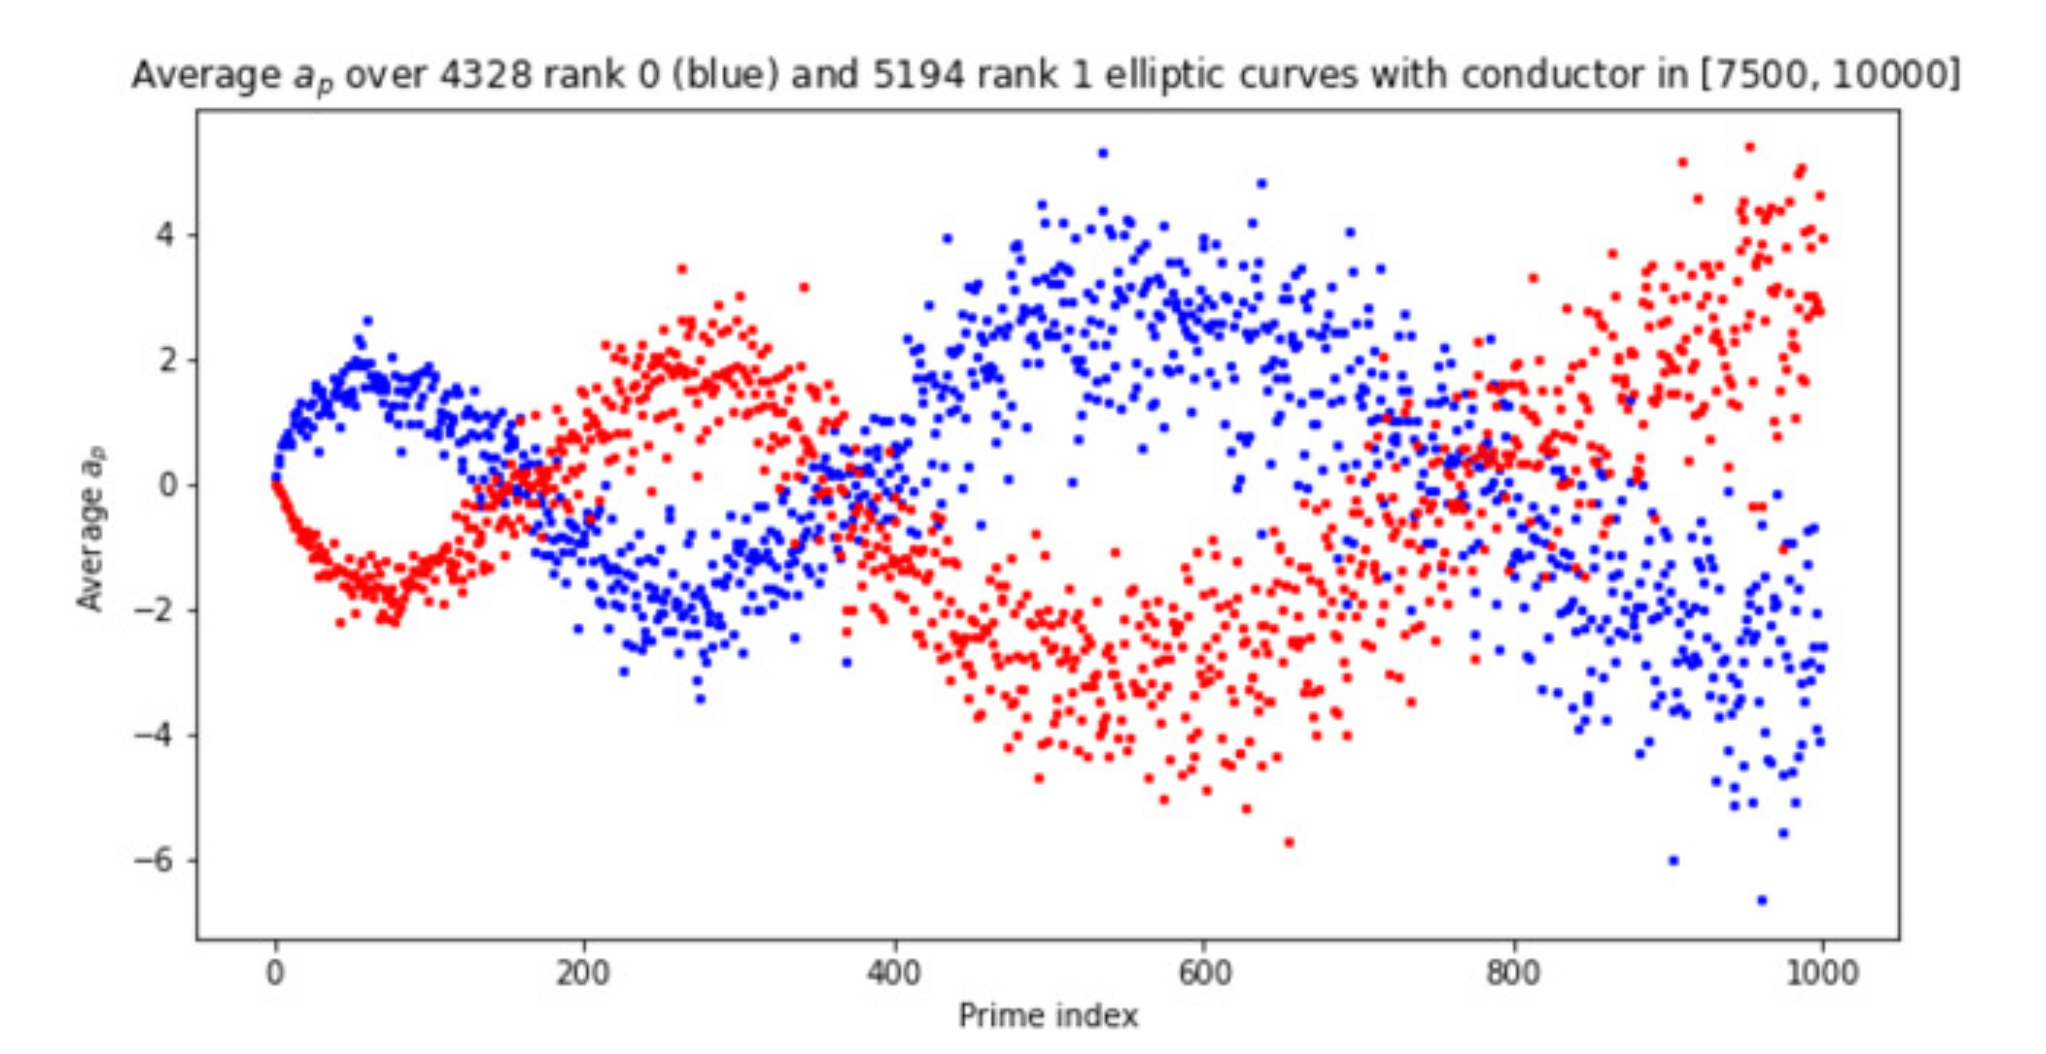
\includegraphics[width=0.7\textwidth]{src/hlop.png}%
    \caption{Murmuration of elliptic curves with conductor in $[7500, 1000]$ and rank $r = 0$ (blue) and $r = 1$ (red) \cite{he2024murmurations}.}
\label{fig:hlop}
\end{figure}


\subsection{Sutherland's observation}
\label{subsec:elliptic_sutherland}

Later, Sutherland \cite{sutherlandletter} (and further work by several people) showed that one really needs to view the murmuration density as a function of $p / N$ rather than $p$ for a fixed $N$.
He found that, for different dyadic intervals of the form $(2^k, 2^{k+1}]$, the murmuration patterns look the same (and become clearer as $k$ increases), even if the averages consider completely different sets of elliptic curves (Figure \ref{fig:sutherland_elliptic_dyadic}).
Also, instead of considering each rank separately, it seems better to consider all ranks together, where we weight $a_p(E)$ by the root number $\epsilon(E)$ of $E$.
One can separate into two groups depending on the parity of the rank.
So the major open question is to \emph{compute} the density function, i.e., to find a function $M: (0, \infty) \to \bR$ such that
\begin{equation}
    \bE_{E \in \cE_r[N, 2N]} [a_p(E)] = M\left(\frac{p}{N}\right) + \text{error}
\end{equation}
where the error term goes to zero as $N \to \infty$. More generally, one can fix $0 < C_1 < C_2$ and consider the interval $[C_1 N, C_2 N]$.

\begin{figure}[htp] 
    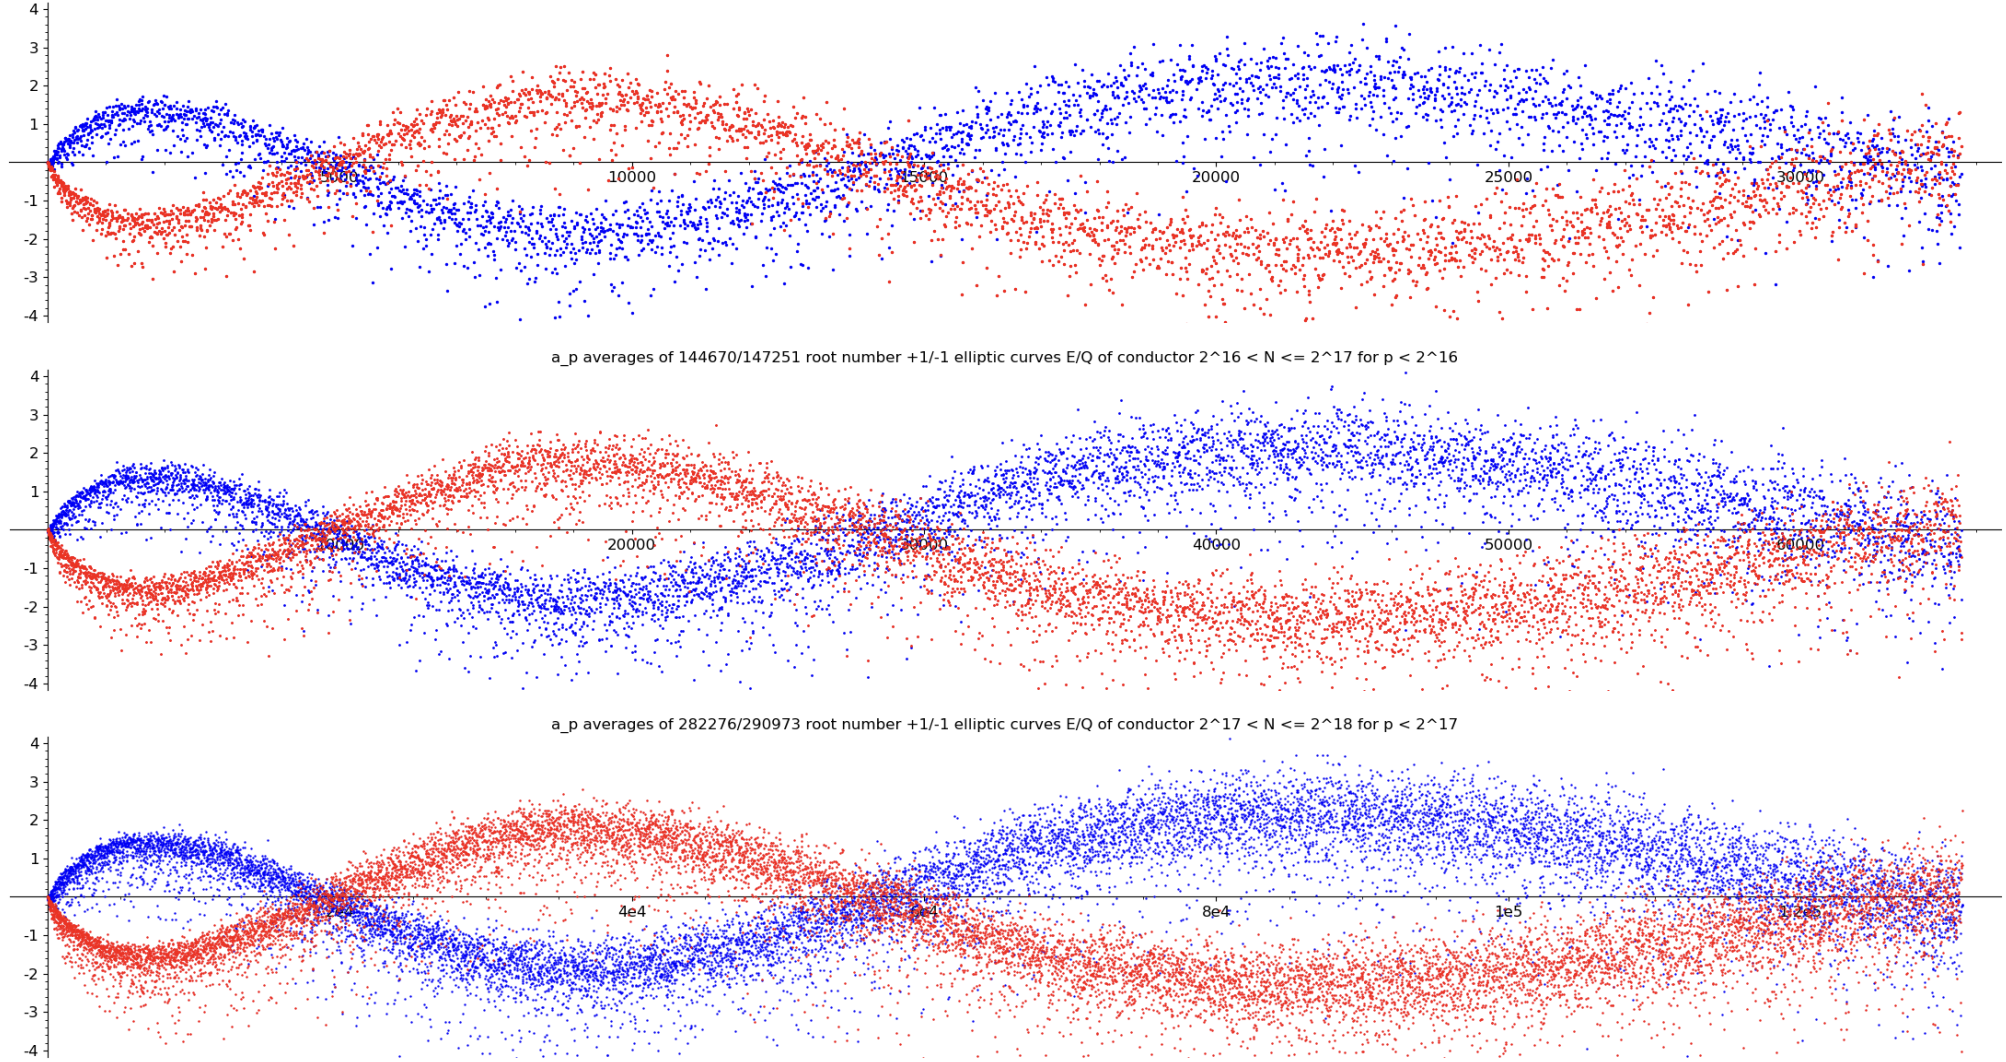
\includegraphics[width=\textwidth]{src/sutherland.png}%
    \caption{Murmuration of elliptic curves with conductor in $[2^{k}, 2^{k+1})$ and primes $p < 2^{k-1}$ for $k = 15, 16, 17$ \cite{sutherlandletter}. Blue (resp. red) curves correspond to $\epsilon(E) = +1$ (resp. $-1$) elliptic curves.}
\label{fig:sutherland_elliptic_dyadic}
\end{figure}


Sutherland also observed that the murmuration disappears when elliptic curves are ordered by other measures, such as naive height, discriminant, or $j$-invariants, although further local averaging gives murmuration for naive heights (see Section \ref{sec:elliptic2}).
This shows that the murmuration is a phenomenon that is sensitive to the ordering of elliptic curves.


\subsection{What is the role of Machine Learning?}

Although there seems to be no machine learning involved in the previous discussions, I will make a brief comment on the relation between machine learning and murmuration, as I found that existing literature is often misleading in distinguishing the machine learning part from the murmuration part.
I have read a few articles on the internet which basically say that ``AI found new mathematics,'' which is false.

One of the main motivations of the paper \cite{he2024murmurations} is to study elliptic curves via machine learning.
In particular, they were interested in predicting the rank of elliptic curves (which is widely known to be hard to compute in general) by means of machine learning, where the coefficients $a_p(E)$ of Hasse--Weil $L$-functions are used as features.
Surprisingly, they found that a simple logistic regression model can already distinguish between rank $0$ and $1$ elliptic curves with high accuracy of $>90\%$ (see also \cite{he2023machine}).
Along these lines, they (more precisely, He, Lee, and Oliver) were curious about what was actually going on, and Pozdnyakov (who was an undergraduate student of Lee at that time) figured out the murmuration pattern.
This somehow gives an explanation for the high accuracy of the model, since the murmuration patterns for rank $0$ and $1$ elliptic curves are noticeably different.
But the correct way to say it is that the machine learning experiments \emph{motivated} them to study what the models were doing, which is essentially the work of humans, not the ML models.
You can find more of the story in the Quanta Magazine article \cite{chiou2024elliptic}.

% and they conjectured that the murmuration density is related to the rank of elliptic curves.

\subsection{Sato--Tate conjecture and Murmuration}


One should not confuse murmuration with the (vertical) Sato--Tate conjecture, which we will explain here.
The original (i.e., \emph{horizontal}) Sato--Tate conjecture is about the distribution of $a_p(E)$ for a \emph{fixed $E_{/\bQ}$ and varying $p$}.
The Hasse--Weil bound says that $|a_p(E)| \le 2 \sqrt{p}$, and the conjecture predicts that for a non-CM elliptic curve $E$, the distribution of $a_p(E)$ is semicircular with radius $2\sqrt{p}$, i.e., the density function is $\frac{1}{2\pi}\sqrt{4 - x^2} \dd x$ for the normalized traces $a_p(E)/\sqrt{p}$.
Equivalently, if we write $a_p(E) = 2 \sqrt{p} \cos \theta_p$ for $\theta_p \in [0, \pi]$, then $\theta_p$ follows the distribution $\frac{2}{\pi} \sin^2 \theta \dd \theta$.
The distributions for CM elliptic curves are different, and we also expect that the Frobenius traces for abelian varieties of higher dimension will follow certain distributions, which are conjecturally the pushforward of the Haar measure of a certain compact Lie group, called the \emph{Sato--Tate group}.
See \cite{sutherland2019sato} for more about the Sato--Tate conjecture and recent progress on it.


The \emph{vertical} Sato--Tate conjecture fixes $p$ and varies $E$ over $\bF_p$ instead, where there are only finitely many isomorphism classes of $E$ over $\bF_p$.
Birch \cite{birch1968number} proved that the distribution converges to the above semicircular distribution as $p \to \infty$.
This is different from the murmuration for two reasons: vertical Sato--Tate considers the elliptic curves over $\bF_p$, and there's no conductor involved in vertical Sato--Tate.

Probably, a closer situation would be fixing a prime $p$ and varying $E$ over $\bQ$ with conductors in a certain range.
Although we couldn't find a reference for this direction, the most relevant case would be the corresponding case of modular forms by Serre \cite{serre1997repartition}.
In particular, he proved that: if a sequence of pairs of weight and level $(k_i, N_i)$ satisfies $2 \mid k_i$, $k_i + N_i \to \infty$, and $p \nmid N_i$, then the distribution of the normalized Hecke eigenvalues $a_p / p^{\frac{k-1}{2}} \in [-2, 2]$ converges to the Plancherel measure
\[
\mu_p = \frac{p+1}{2\pi} \frac{\sqrt{4 - x^2}}{(p^{\frac{1}{2}} + p^{-\frac{1}{2}})^2 - x^2} \dd x.
\]
Hence one can fix weight $k = 2$ and vary the level $N \to \infty$ with $p \nmid N$.
However, this includes many more modular forms than the ones corresponding to elliptic curves.
Also, we want both $p$ and $N$ to grow at similar rates in murmuration, so Serre's result does not directly apply to our situation.
\section{Murmuration of Dirichlet Series}

Although the original murmuration density for elliptic curves is still unknown, there are a few works where murmuration exists and is even computed (under GRH).
Historically, the first such example is the work of Zubrilina on modular forms \cite{zubrilina2025murmurations}, but we will start with the simplest case of Dirichlet characters.
Lee, Oliver, and Pozdnyakov computed the murmuration density for Dirichlet characters \cite{lee2025murmurations}\footnote{These can be thought of as automorphic forms on $\GL_1$ over $\bQ$.}.
For complex characters, the corresponding murmuration densities are given by the following theorem.

\begin{theorem}[{Lee--Oliver--Pozdnyakov \cite[Theorem 1.1]{lee2025murmurations}}]
    \label{thm:lop_dirichlet}
    Let $\cD_{+}(N)$ (resp. $\cD_{-}(N)$) denote the set of primitive even (resp. odd) Dirichlet characters modulo $N$.
    For $x \in \bR_{> 0}$, let $\lceil x \rceil^{\frp}$ be the smallest prime $\ge x$.
    For $c > 1$, $\delta > 0$, and $y > 0$, define
    \begin{align}
        P_{\pm}(y, X, c) &:= \frac{\log X}{X} \sum_{\substack{N \in [X, cX] \\ N \text{ prime}}} \sum_{\chi \in \cD_{\pm}(N)} \frac{\chi(\lceil yX \rceil^{\frp})}{\tau(\chi)}, \label{eqn:lee_1_avg} \\
        P_{\pm}(y, X, \delta) &:= \frac{\log X}{X^\gamma} \sum_{\substack{N \in [X, X + X^\gamma] \\ N \text{ prime}}} \sum_{\chi \in \cD_{\pm}(N)} \frac{\chi(\lceil yX \rceil^{\frp})}{\tau(\chi)}. \label{eqn:lee_2_avg}
    \end{align}
    Then
    \begin{equation}
        \label{eqn:lee_1}
        \lim_{X \to \infty} P_{\pm} (y, X, c) = \begin{cases}
            \int_{1}^{c} \cos\left(\frac{2 \pi y}{x}\right) \dd x & \text{if } +, \\
            -i \int_{1}^{c} \sin \left(\frac{2 \pi y}{x}\right) \dd x & \text{if } -,
        \end{cases}
    \end{equation}
    and assuming RH, if $\frac{1}{2} < \gamma < 1$, we have
    \begin{equation}
        \label{eqn:lee_2}
        \lim_{X \to \infty} P_{\pm} (y, X, \gamma) = \begin{cases}
            \cos (2 \pi y) & \text{if } +, \\
            -i \sin (2 \pi y) & \text{if } -.
        \end{cases}
    \end{equation}
\end{theorem}

See Figure \ref{fig:lop} for the plot of the above murmuration densities.
As you can see, there are two versions of murmurations: the \emph{long interval} $[X, cX]$ and the \emph{short interval} $[X, X + X^\delta]$.
Note that one needs to assume RH to get the short interval version, to guarantee the existence of primes in short intervals.
The summand $\chi(p) / \tau(\chi)$ is the $p$-th Fourier coefficient of $\overline{\chi}$ when expanded in terms of additive characters: we have \cite[eq. (3.12)]{iwaniec2021analytic}
\[
\overline{\chi}(a) = \frac{1}{\tau(\chi)} \sum_{b \Mod N} \chi(b) \exp\left(\frac{2 \pi i ab}{N}\right)
\]
when $\tau(\chi) \ne 0$, which justifies the normalization (Note that $\cD_\pm(N)$ is invariant under complex conjugation).
Also, the above averages only consider prime moduli, though the authors also studied the case of composite moduli in \cite[Section 6.1]{lee2025murmurations}.

The proof of Theorem \ref{thm:lop_dirichlet} is much simpler than the case of modular forms (Section \ref{sec:modform}).
By orthogonality of characters, we have
\[
\exp\left(\frac{2 \pi i a}{N}\right) = \cos\left(\frac{2 \pi a}{N}\right) + i \sin\left(\frac{2 \pi a}{N}\right) = \frac{1}{\phi(N)} \sum_{\chi \Mod N} \overline{\chi}(a) \tau(\chi)
\]
and taking $a = p$ and $-p$ for a prime $p \nmid N$ gives (note that $\tau(\chi_0) = -1$)
\begin{align*}
    \cos \left(\frac{2\pi p}{N}\right) &= -\frac{1}{\phi(N)} + \frac{1}{\phi(N)} \sum_{\substack{\chi\Mod N \\ \chi \ne \chi_0,\,\chi(-1) = 1}} \tau(\overline{\chi}) \chi(p), \\
    \sin \left(\frac{2 \pi p}{N}\right) &= - \frac{i}{\phi(N)} \sum_{\substack{\chi \Mod N \\ \chi(-1) = -1}} \tau(\overline{\chi}) \chi(p).
\end{align*}
Now, use $\tau(\chi) \tau(\overline{\chi}) = N \chi(-1)$ for $\chi \in \cD_{\pm}(N)$ to get \cite[Lemma 2.6]{lee2025murmurations}: for two distinct primes $p$ and $N$,
\begin{align*}
    \sum_{\chi \in \cD_{+}(N)} \frac{\chi(p)}{\tau(\chi)} &= \left(\frac{N-1}{N}\right) \cos \left(\frac{2 \pi p}{N}\right) + \frac{1}{N}, \\
    \sum_{\chi \in \cD_{-}(N)} \frac{\chi(p)}{\tau(\chi)} &= -i\left(\frac{N-1}{N}\right) \sin \left(\frac{2 \pi p}{N}\right).
\end{align*}
Combined with the prime number theorem (which gives equidistribution results of primes in $[X, cX]$ normalized by $X$), we get \eqref{eqn:lee_1}.
For short intervals, RH and the prime number theorem imply
\[
\lim_{X \to \infty} \frac{\log X}{X^\gamma}\cdot \#\{p \in [yX, yX + X^\gamma]\} = 1,
\]
for $\frac{1}{2} < \gamma < 1$, and this implies \cite[Lemma 2.9]{lee2025murmurations} 
\begin{equation}
\label{eqn:short_avg}
\lim_{X \to \infty} \frac{\log X}{X^\gamma} \sum_{\substack{p \in [yX, yX + X^\gamma] \\ p \text{ prime}}} f\left(\frac{p}{X}\right) = f(y)
\end{equation}
which proves \eqref{eqn:lee_2}.

They also proved similar results for real Dirichlet characters, but the proof is more complicated.
Let $\scG$ be the set of odd square-free integers and let $\chi_{d} = \left(\frac{d}{\cdot}\right)$.
For a compactly supported smooth function $\Phi \ge 0$ on $\bR$, define
\begin{equation}
    M_{\Phi}(y, X, \gamma) = \frac{\log X}{X^{1 + \gamma}} \sum_{\substack{p \in [yX, yX + X^\gamma] \\ p \text{ prime}}} \sum_{d \in \scG} \Phi\left(\frac{d}{X}\right) \chi_{8d}(p) \sqrt{p}.
\end{equation}

\begin{theorem}[{Lee--Oliver--Pozdnyakov \cite[Theorem 1.2]{lee2025murmurations}}]
    \label{thm:lop_dirichlet_quad}
    Fix $y > 0$ and assume $\frac{3}{4} < \gamma < 1$.
    Assuming GRH, we have
    \begin{equation}
        \label{eqn:lop_murm_quad}
        M_{\Phi} (y) := \lim_{X \to \infty} M_{\Phi}(y, X, \gamma) = \frac{1}{2} \sum_{\substack{a \ge 1 \\ a \text{ odd}}} \frac{\mu(a)}{a^2} \sum_{m \ge 1} (-1)^{m} \widetilde{\Phi} \left(\frac{m^2}{2 a^2 y}\right),
    \end{equation}
    where
    \begin{equation}
        \widetilde{\Phi}(\xi) = \int_{-\infty}^{\infty} (\cos(2 \pi \xi x) + \sin(2 \pi \xi x)) \Phi(x) \dd x.
    \end{equation}
    (The limit does not depend on the choice of $\gamma$.)
\end{theorem}
% The authors also considered the case of $\chi_d$; see \cite[Section 6.2]{lee2025murmurations}.
See Figure \ref{fig:lop_quad} for the corresponding plots when $\Phi_+$ (resp. $\Phi_-$) is supported on $(1, 2)$ (resp. $(-2, -1)$).
For the proof, we can write $M_\Phi(y, X, \gamma)$ as
\begin{align*}
    M_\Phi(y, X, \gamma) &= \frac{\log X}{X^{1 + \gamma}} \sum_{\substack{p \in [yX, yX + X^\gamma] \\ p \text{ prime}}} \sum_{\substack{d \in \bZ \\ d \text{ odd}}} \mu^2(d) \Phi\left(\frac{d}{X}\right) \chi_{8d}(p) \sqrt{p} \\
    &= \frac{\log X}{X^{1 + \gamma}} \sum_{\substack{p \in [yX, yX + X^\gamma] \\ p \text{ prime}}} \sum_{\substack{d \in \bZ \\ d \text{ odd}}} \left(\sum_{\substack{a^2 \mid d \\ 0 < a}}\mu(a)\right) \Phi\left(\frac{d}{X}\right) \chi_{8d}(p) \sqrt{p} \\
    &= M_{\Phi, A}(y, X, \gamma) + R_{\Phi, A}(y, X, \gamma),
\end{align*}
where $\beta := \sup_{x \in \bR}\{|x|: \Phi(x) > 0\}$, $0 < A \le \sqrt{\beta X}$, and
\begin{align}
    M_{\Phi, A}(y, X, \gamma) &:= \frac{\log X}{X^{1 + \gamma}} \sum_{\substack{p \in [yX, yX + X^\gamma] \\ p \text{ prime}}} \sum_{\substack{d \in \bZ \\ d \text{ odd}}} \left(\sum_{\substack{a^2 \mid d \\ 0 < a \le A}}\mu(a)\right) \Phi\left(\frac{d}{X}\right) \chi_{8d}(p) \sqrt{p}, \label{eqn:MA} \\
    R_{\Phi, A}(y, X, \gamma) &:= \frac{\log X}{X^{1 + \gamma}} \sum_{\substack{p \in [yX, yX + X^\gamma] \\ p \text{ prime}}} \sum_{\substack{d \in \bZ \\ d \text{ odd}}} \left(\sum_{\substack{a^2 \mid d \\ A < a}}\mu(a)\right) \Phi\left(\frac{d}{X}\right) \chi_{8d}(p) \sqrt{p}. \label{eqn:RA}
\end{align}
We will show that $R_{\Phi, A}(y, X, \gamma) \to 0$ and $M_{\Phi, A}(y, X, \gamma)$ converges to the right-hand side of \eqref{eqn:lop_murm_quad}.
Note that $A$ will not be a fixed constant, but rather grows together with $X$: in fact, the proof uses $0 < \epsilon < (\delta - \frac{3}{4}) / 5$ and $A = X^{1 + 5 \epsilon - \delta}$.
By applying the Polya--Vinogradov inequality
\begin{equation}
    \label{eqn:pv}
    \left|\sum_{\substack{p \in [yX, yX + X^\gamma] \\ p\text{ prime}}} \chi_d(p)\right| \ll (yX)^{\frac{1}{2} + \epsilon}
\end{equation}
for non-principal $\chi_d$ and $\frac{1}{2} < \gamma < 1$ (which uses GRH \cite{granville2007large}), and Abel's summation formula, one can show that the remainder term $R_{\Phi, A}(y, X, \gamma)$ vanishes as $X \to \infty$, where $\gamma > \frac{3}{4}$ is used in the computation.
For the main term $M_{\Phi, A}(y, X, \gamma)$, the Poisson summation formula implies \cite[Lemma 2.11]{lee2025murmurations}
\[
\frac{1}{X} \sum_{\substack{d \in \bZ \\ d \text{ odd}}} \left(\sum_{\substack{a^2 \mid |d| \\ a \le A}} \mu(a)\right) \Phi\left(\frac{d}{X}\right) \left(\frac{d}{p}\right) \sqrt{p} = \frac{1}{2} \left(\frac{2}{p}\right) \sum_{\substack{0 < a \le A \\ (a, 2p) = 1}} \frac{\mu(a)}{a^2} \sum_{k \in \bZ} (-1)^k \left(\frac{k}{p}\right) \widetilde{\Phi} \left(\frac{k X}{2 a^2 p}\right),
\]
and applying it to \eqref{eqn:MA} gives
\[
M_{\Phi, A}(y, X, \gamma) = \frac{\log X}{X^\gamma} \sum_{\substack{p \in [yX, yX + X^\gamma] \\ p \text{ prime}}} \frac{1}{2} \sum_{\substack{0 < a \le A \\ (a, 2p) = 1}} \frac{\mu(a)}{a^2} \sum_{0 \ne k \in \bZ} (-1)^k \left(\frac{k}{p}\right) \widetilde{\Phi} \left(\frac{k X}{2 a^2 p}\right)
\]
for sufficiently large $X$.
Since $0 < a \le A \ll X^{\frac{1}{2}} \ll p$, we have $(a, 2p) = 1$ if and only if $(a, 2) = 1$, and switching the order of summation gives
\[
M_{\Phi, A}(y, X, \gamma) = \frac{1}{2} \sum_{\substack{(a,2) = 1 \\ 0 < a \le A}} \frac{\mu(a)}{a^2} \sum_{0 \ne k \in \bZ} (-1)^k \frac{\log X}{X^\gamma} \sum_{\substack{p \in [yX, yX + X^\gamma] \\ p \text{ prime}}} \left(\frac{k}{p}\right) \widetilde{\Phi} \left(\frac{k X}{2 a^2 p}\right).
\]
Now, using the Polya--Vinogradov inequality \eqref{eqn:pv} again, one can show that the summation over non-square $k$ exhibits cancellation and only the sum over square $k$ contributes to the main term ($\gamma > \frac{3}{4}$ is used again):
\[
\lim_{X \to \infty} M_{\Phi, A}(y, X, \gamma) = \lim_{X \to \infty} \frac{\log X}{X^\gamma} \sum_{\substack{p \in [yX, yX + X^\gamma] \\ p \text{ prime}}} \frac{1}{2} \sum_{\substack{(a,2) = 1 \\ 0 < a \le A}} \frac{\mu(a)}{a^2} \sum_{\substack{m \ge 1 \\ (m, p) = 1}} (-1)^m \widetilde{\Phi} \left(\frac{m^2 X}{2 a^2 p}\right).
\]
Finally, one can use the Poisson summation formula to show that the two inner sums on the right-hand side converge to a smooth function in $y = p / X$ as $X \to \infty$ (hence $A \to \infty$), and applying \eqref{eqn:short_avg} gives the desired result.


\begin{figure}[htp] 
\centering
    \begin{subfigure}{1.0\textwidth}
        \centering
        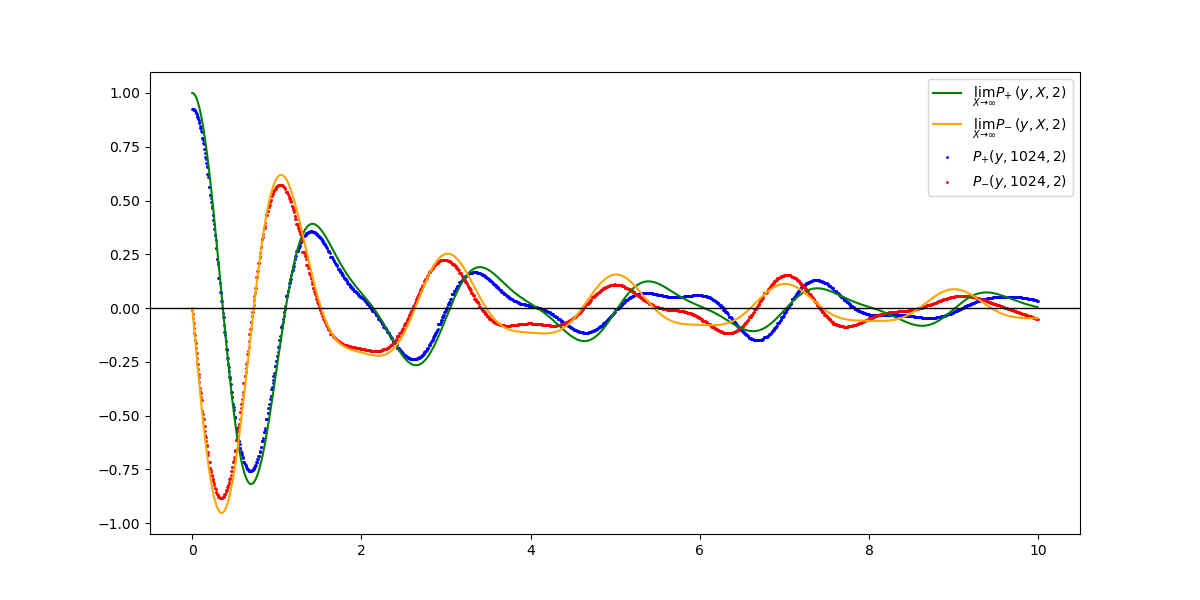
\includegraphics[width=\textwidth]{src/lop_fig1_top.png}%
        \label{fig:lop_fig1_top}
    \end{subfigure}
    
    \begin{subfigure}{1.0\textwidth}
        \centering
        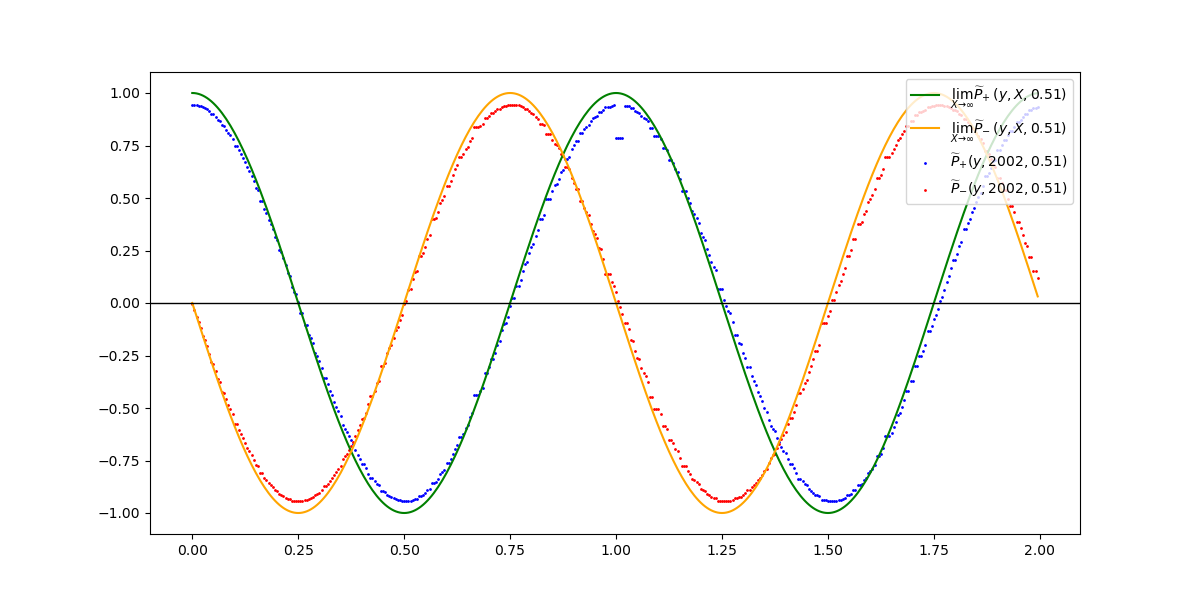
\includegraphics[width=\textwidth]{src/lop_fig1_bottom.png}%
        \label{fig:lop_fig1_bottom}
    \end{subfigure}

    \caption{Murmuration of Dirichlet characters. The top figure presents $P_{\pm}(y, 2^{10}, 2)$ for $y \in [0, 10]$ with $+$ in blue and (the imaginary part of) $-$ in red. The bottom figure presents $\widetilde{P}_{\pm}(y, 2002, 0.51)$ for $y \in [0, 2]$ with $+$ in blue and (the imaginary part of) $-$ in red. The discontinuity of $\widetilde{P}_{+}(y, 2002, 0.51)$ at $y = 1$ corresponds to the term $p = N$ in \eqref{eqn:lee_2_avg}.}
\label{fig:lop}
\end{figure}


\begin{figure}[htp] 
\centering
    \begin{subfigure}{1.0\textwidth}
        \centering
        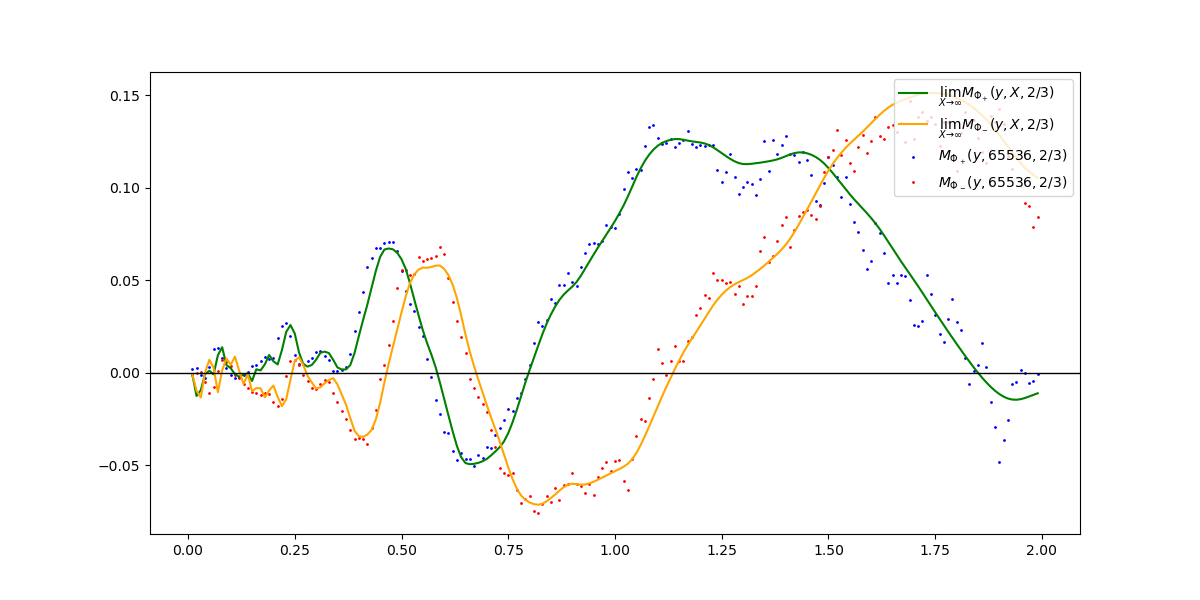
\includegraphics[width=\textwidth]{src/lop_fig2.png}%
        \label{fig:lop_fig2}
    \end{subfigure}
    
    \begin{subfigure}{1.0\textwidth}
        \centering
        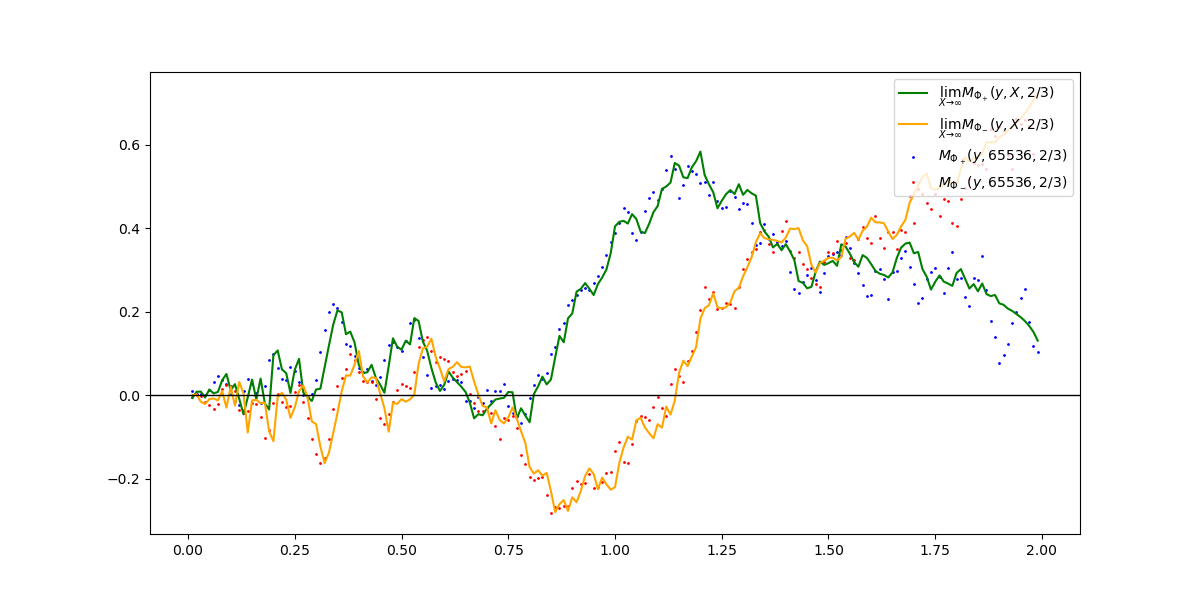
\includegraphics[width=\textwidth]{src/lop_fig3.png}%
        \label{fig:lop_fig3}
    \end{subfigure}

    \caption{Murmuration of Kronecker characters $\chi_{8d}$. The top figure presents $M_{\Phi_{\pm}}(y, 2^{16}, \frac{2}{3})$ for $y \in [0, 2]$ with $\Phi_+(x) = \1_{(1, 2)}(x) \exp(-1/(1 - 4(x - \frac{3}{2})^2))$ and $\Phi_-(x) = \1_{(-2, -1)}(x) \exp(-1/(1 - 4(x + \frac{3}{2})^2))$. The bottom figure presents $M_{\Phi_{\pm}}(y, 2^{16}, \frac{2}{3})$ for $y \in [0, 2]$ with $\Phi_+(x) = \1_{(1, 2)}(x)$ and $\Phi_-(x) = \1_{(-2, -1)}(x)$. Note that we use $\gamma = \frac{2}{3}$, even if the above proof only works when $\gamma > \frac{3}{4}$.}
\label{fig:lop_quad}
\end{figure}
\section{Murmuration of Modular Forms}
\label{sec:modform}

The first murmuration density that is computed ever is for modular forms by Zubrilina \cite{zubrilina2023murmurations}.

\subsection{Statement}

Before we state the result, we define some notations first.
\begin{itemize}
    \item For $n \in \bZ_{\ge 0}$, \emph{Chebyshev polynomial of the second kind} is defined as
    \[
        U_n(\cos \theta) = \frac{\sin((n+1) \theta)}{\sin\theta}. 
    \]
    \item For $r \in \bZ_{\ge 1}$, define
    \[
        \nu(r) := \prod_{p | r} \left(1 + \frac{p^2}{p^4 - 2p^2 - p + 1}\right)
    \]
    \item Define constants $\alpha, \beta, \gamma$ as
    \begin{align*}
        \alpha &:= 2\pi \prod_{p} \frac{p^4 - 2p^2 - p + 1}{p^4 - 2p^2 + p}, \\
        \beta &:= 2\pi \prod_{p} \frac{p^3 + p^2 - 1}{p(p^2 + p - 1)}, \\
        \gamma &:= 12 \prod_{p} \frac{p(p + 1)}{p^2 + p - 1}.
    \end{align*}
\end{itemize}
\begin{theorem}[Zubrilina {\cite{zubrilina2023murmurations}}]
    \label{thm:zubrilina_modform}
    Let $X, Y, P$ be parameters going infinite with $X, Y > 0$ and $P$ prime; assume further that $Y = (1 + o(1))X^{1 - \delta_2}$ and $P \ll X^{1 + \delta_1}$ for some $\delta_1, \delta_2$ with $2\delta_1 < \delta_2 < 1$.
    Let $y = P/X$. Then
    \begin{equation}
        \label{eqn:zubrilina_modform}
        \frac{\sum_{N \in [X, X + Y]}^\square \sum_{f \in H^{\new}(N, k)} \sqrt{P} \lambda_f(P) \varepsilon(f)}{\sum_{N \in  [X, X + Y]}^\square \sum_{f \in H^{\new}(N, k)} 1} = \cM_k(y) + O_\varepsilon \left(X^{-\delta' + \varepsilon} + \frac{1}{P}\right)
    \end{equation}
    where
    \begin{equation}
        \cM_k(y) = \frac{\alpha(-1)^{k/2 - 1}}{k - 1} \sum_{1 \le r \le 2\sqrt{y}} \nu(r) \sqrt{4y - r^2} U_{k - 2} \left(\frac{r}{2\sqrt{y}}\right) + \frac{\beta}{k-1} \sqrt{y} - \gamma \delta_{k=2} y.
    \end{equation}
\end{theorem}

\subsection{Eichler--Selberg trace formula}

To prove Theorem \ref{thm:zubrilina_modform}, one need to understand how to estimate the numerator on the LHS.
Recall that $a_f(P) = P^{(k-1)/2} \lambda_f(P)$ is the $P$-th Fourier coefficient of $f$, which is also the eigenvalue of the Hecke operator $T_P$ acting on $f$.
Also, $(-1)^{k/2}\varepsilon(f)$ is equal to the eigenvalue of the Atkin--Lehner involution $W_N = T_N$ acting on $f$.
Thus the sum appears in the numerator of LHS of \eqref{eqn:zubrilina_modform} can be interpreted as the trace of the operator $(-1)^{k/2} T_P \circ W_N$ acting on the space of cusp forms of weight $k$ and level $N$ (multiplied by $P^{1 - k/2}$).
Eichler \cite{eichler1955class} studied such a sum of traces and proved that it can be expressed in terms of (Hurwitz) class numbers, which is generalized by Selberg \cite{selberg1956harmonic}.
To account the root number $\varepsilon(f)$, i.e. eigenvalue of $W_N$, we used the following version of Eichler--Selberg trace formula by Skoruppa and Zagier \cite{skoruppa1987jacobi}.

\begin{theorem}[Skoruppa--Zagier \cite{skoruppa1987jacobi}]
    \label{thm:sz_tf}
    For square-free $N$ and prime $P \nmid N$,
    \begin{align*}
        &\sum_{f \in H^\new(N, k)} \sqrt{P} \lambda_f(P) \varepsilon(f)\nonumber \\
        &= \frac{H_1(-4PN)}{2} + (-1)^{k/2 - 1} U_{k - 2} \left(\frac{r\sqrt{N}}{2\sqrt{P}}\right) \sum_{0 < r \le 2\sqrt{P/N}} H_1(r^2 N^2 - 4PN) \\
        &\quad - \delta_{k-2}(P+1)
    \end{align*}
    Here $H_1(-d)$ ($d > 0$) is the Hurwitz class number, the number of equivalence classes of positive definite binary quadratic forms of discriminant $-d$ weighted by the number of automorphisms, i.e. with forms correspond to $x^2 + y^2$ or $x^2 + xy + y^2$ counted with multiplicity $1/2$ and $1/3$ respectively.
\end{theorem}

Hurwitz class number can be expressed as a sum of usual class numbers as
\[
H_1(-d) = \sum_{f^2 | d} h(-d / f^2) + O(1)
\]
where the ``error term'' $O(1)$ disappears if $d \ne 3 \cdot \square$ or $4 \cdot \square$.
Using this, we can rewrite the Skoruppa--Zagier trace formula as
\begin{align*}
    &\sum_{f \in H^\new(k, N)} \sqrt{P} \lambda_f(P) \varepsilon(f) \\
    &= \frac{h(-4PN)}{2} + \frac{h(-PN)}{2} - \delta_{k=2} P + O(1) \\
    &+ (-1)^{k/2 - 1} U_{k-2} \left(\frac{r\sqrt{N}}{2\sqrt{P}}\right) \sum_{1 \le r \le 2\sqrt{P/N}} \sum_{d^2 | r^2 N - 4P} h\left(\frac{N(r^2 N - 4P)}{d^2}\right)
\end{align*}

From this, our new goal is to estimage the average of class numbers over short intervals, i.e. when $N \in [X, X + Y]$ with $Y = o(X)$.
The main idea is to use class number formula to write class numbers as special $L$-values at $s = 1$, e.g.
\[
h(-d) = \frac{\sqrt{d}}{\pi} L(1, \chi_d)
\]
when $d > 4$ and $-d \equiv 1 \Mod{4}$.
Then the sum (average) of the corresponding $L$-values can be estimated via truncation and Polya--Vinogradov inequality.
For example, we have an estimate
\[
L(1, \chi_d) = \sum_{n \ge 1} \frac{\chi_d(n)}{n} = \sum_{1 \le n \le T} \frac{\chi_d(n)}{n} + O\left(\frac{\sqrt{d} \log d}{T}\right).
\]
With some hard analysis, one get the following estimations.
\begin{proposition}[Zubrilina {\cite[Proposition 3.1]{zubrilina2023murmurations}}]
    Let $P$ be an odd prime and let $[X, X + Y]$ be an interval with $Y = o(X)$.
    Then as $X \to \infty$,
    \begin{align*}
        &\frac{\zeta(2) \pi}{XY} \sideset{}{{}^\square}\sum_{\substack{N \in [X, X + Y] \\ P \nmid N}}  \left(\frac{h(-PN)}{2} + \frac{h(-4PN)}{2} \right) \\
        &= A \sqrt{y} + O_{\varepsilon} \left(\frac{1}{P^{3/2}X^{1/2}} + \frac{P^{7/12}}{Y^{5/6} X^{5/12}} + \frac{YP^{1/2}}{X^{3/2}}\right) (XYP)^{\varepsilon}
    \end{align*}
\end{proposition}


\begin{proposition}[Zubrilina {\cite[Proposition 3.2]{zubrilina2023murmurations}}]
    Let $P$ be an odd prime, $r \in \bN$, and $X > Y > 0$ be such that $r^2(X + Y) < 4 P$ for each $r > 2 \sqrt{P/X}$. Let $y = P/X$. Then
    \begin{align*}
        &\frac{\zeta(2) \pi}{ XY} \sum_{r \le 2 \sqrt{P/X}} \,\,\,\, \sideset{}{{}^\square}\sum_{\substack{N \in [X, X + Y] \\ P \nmid N}}  H_1\left(r^2 N^2 - 4 PN\right) \\
        &= \sum_{r \le 2 \sqrt{P/X}} \nu(r) \sqrt{4y - r^2} \\
        &+ O\left(\frac{P^{11/10}}{Y^{2/5}X^{9/10}} + \frac{YP}{X^2} + \frac{PY^{1/2}}{X^{3/2}} + \frac{P}{X^{1/2} Y^{13/18}} + \frac{P}{XY^{1/9}}\right) (XYP)^\varepsilon
    \end{align*}
\end{proposition}

\subsection{Doesn't Zubrilina's result prove murmuration for elliptic curves, because of the modularity?}

\emph{No!} I was also confused about this.
The reason is because elliptic curves over $\bQ$ corresponds to modular forms of weight $2$ \emph{with coefficient field (Hecke field) $\bQ$} (recall that $a_p(E) = p + 1 - \#E(\bF_p)$ are integers).
The family (see also Section \ref{subsec:other_sarnak}) that Zubrilina considered is much larger than the family of elliptic curves in \cite{he2024murmurations}, and it seems hard to isolate such family from whole family of Hecke eigenforms (of weight 2).
It is conjectured that the \emph{conductor dimension} (See \ref{subsec:other_sarnak} for the definition) of elliptic curves is $\frac{5}{6}$ \cite{shankar2019families}, while that of weight 2 modular forms is $2$.
\section{Murmuration of Elliptic Curves, Revisited}
\label{sec:elliptic2}

Recently, Will Sawin and Andrew Sutherland announced a murmuration theorem for elliptic curves \cite{sawin2025murmurations}, which is slightly different from the formulation in \cite{he2024murmurations}.
Especially, they proved a version of the murmuration theorem \emph{ordered by height}:


\begin{theorem}[Sawin--Sutherland {\cite{sawin2025murmurations}}]
    \label{thm:sawin-sutherland}
    Let 
    \[
    \scE(X) := \{y^2 = x^3 + ax + b: a, b \in \bZ, p^4 \mid a \Rightarrow p^6 \nmid b, \max\{4|a|^3, 27 b^2\} \le X\}
    \]
    be the set of isogenous classes of elliptic curves over $\bQ$ ordered by naive height.
    For any smooth function $W : \bR_{>0} \to \bR$ with compact support, the limit
    \begin{equation}
        \lim_{P \to \infty }\lim_{X \to \infty} \bE_{\scE(X)} \left[ \frac{\prod_{p \le P}(1 - p^{-1})^{-1}}{N(E)} \sum_{\substack{n \ge 1 \\ p \nmid n \,\forall p \le P}} W\left(\frac{n}{N(E)}\right) a_n(E) \epsilon(E)\right]
    \end{equation}
    exists and is equal to
    \begin{equation}
        \int_{0}^{\infty} W(u) \sqrt{u} \left(2\pi \sideset{}{{}^\square}\sum_{q \ge 1} \sum_{m \ge 1} \frac{\mu(\gcd(m,q))}{qm \phi\left(\frac{q}{\gcd(m,q)}\right)} J_1 \left(\frac{4 \pi \sqrt{u}m}{q}\right) \prod_{p \mid q} \hat{\ell}_{p, 2v_p(m)} \prod_{p \mid m, p \nmid q} \ell_{p, 2v_p(m)} \right) \dd u
    \end{equation}
    where $\ell_{p, \nu}$ and $\hat{\ell}_{p, \nu}$ are certain local factors that can be written in terms of traces of the Hecke operator $T_p$ (see \cite[Lemma 3, 4]{sawin2025murmurations}).
\end{theorem}

You should have a question at this point.
We said that Sutherland observed no murmuration pattern in \cite{sutherlandletter} when elliptic curves are ordered by height, but Theorem \ref{thm:sawin-sutherland} seems to suggest that there is a murmuration pattern.
In fact, the difference comes from \emph{local averaging}, which I'm going to explain now.

The difference between the original murmuration observed in HLOP \cite{he2024murmurations} and the one in Sawin--Sutherland is well-explained in \cite[Section 1.1]{sawin2025murmurations}.
The original murmuration considered the averages of the form 
\[
\bE_{\substack{N(E) \in [N_1, N_2] \\ \mathrm{rank}(E) = r}} [a_p(E)]
\]
as a function in $p$ for fixed $r, N_1, N_2$ (initially $[N_1, N_2] = [7500, 10000]$ in \cite{he2024murmurations}).
As mentioned earlier, subsequent works (especially \cite{sutherlandletter}) found that we need to view the murmuration density as a function in $p / N$, not $p$.
Also, it seems better to consider all elliptic curves with same root numbers at once, or weight $a_p$ by root numbers.
Hence the reformulated HLOP's murmuration would be
\begin{equation*}
    % \label{eqn:HLOPavg}
    \bE_{\substack{N(E) \in [X, 2X]}} [\epsilon(E) a_p(E)]
\end{equation*}
In \cite{sawin2025murmurations}, the authors mentioned that Bober suggested that one may need \emph{local averaging} in $p$ before we average over different elliptic curves.
\begin{equation*}
    \bE_{N(E) \in [X, 2X]} \left[\bE_{\substack{p \in (C_1 N(E), C_2 N(E)) \\ p \text{ prime}}} [\epsilon(E) a_p(E)]\right]
\end{equation*}

% However, subsequent works found that the dyadic intervals like $[X, 2X]$ or slightly smaller intervals like $[X, X + X^{1 - \delta}]$ for $\delta > 0$ are more appropriate, since it make analysis more tractable and plots smoother.
% Hence the reformulated HLOP's murmuration would be
% \begin{equation}
% \label{eqn:HLOPavg}
% \bE_{\substack{N(E) \in [X, 2X] \\ \mathrm{rank}(E) = r}} [a_p(E)]
% \end{equation}
% Also, later study found that the oscillations would converge to a continuous function in $p / X$, so we can understand \eqref{eqn:HLOPavg} as (1) the limit of $X \to \infty$ with fixed $p / X$ value, or (2) the limit of the average over $p$ with $p / X$ lies in a fixed interval.

% Another subsequent observation is that considering all elliptic curves with different ranks would be better to study, where we weight $a_p(E)$ by the $\epsilon$ factor of $E$.
% Also, rather than $p / X$, the crucial ratio might be $p / N(E)$. In other words, we can consider further averaging over $p$ where $p / N$ lies in a certain interval, such as
% \[
% \bE_{N(E) \in [X, 2X]} \left[ \bE_{p \in (C_1 N(E), C_2 N(E))} [\epsilon(E) a_p(E)]\right]
% \]
% for $0 < C_1 < C_2$.
% Note that it is slightly easier to work with
% \[
% \bE_{N(E) \in [X, 2X]} \left[ \frac{\log \left(N(E)\frac{C_2 - C_1}{2}\right)}{N(E)}\sum_{p \in (C_1 N(E), C_2 N(E))} \epsilon(E) a_p(E)\right]
% \]
% instead of the previous double expectation, where the term $N / \log(N \frac{C_2 - C_1}{2})$ roughly counts the number of primes in the interval $(C_1 N, C_2 N)$.
% What Sawin and Sutherland proved is a naive height variation of the above average.

The main idea of the proof of Theorem \ref{thm:sawin-sutherland} is the Voronoi summation formula.

\begin{theorem}[{\cite[Lemma 11]{sawin2025murmurations}}]
    Let $E_{/\bQ}$ be an elliptic curves, $q$ be a positive integer, $a$ a positive integer coprime to $q$, and $W: (0, \infty) \to \bR$ a smooth function with compact support.
    Then
    \begin{equation}
        \epsilon(E) \sum_{n \ge 1} \frac{a_n(E)}{\sqrt{n}} W\left(\frac{n}{N(E)}\right) e\left(\frac{an}{q}\right) = \frac{\sqrt{N(E)}}{q} \sum_{n \ge 1} \frac{a_n(E)}{\sqrt{n}} e\left(\frac{\overline{aN(E)} n}{q}\right) \int_0^{\infty} 2 \pi W(u) J_1\left(\frac{4 \pi \sqrt{u}n}{q}\right) \dd u
    \end{equation}
    where $e(x) = e^{2 \pi i x}$ and $\overline{aN(E)}$ is the multiplicative inverse of $aN(E)$ modulo $q$.
\end{theorem}
Note that summation of $n$ instead over primes is built-in inside the formula.
Based on the theorem, they also conjectured that:

\begin{conjecture}[{\cite[Conjecture 1]{sawin2025murmurations}}]
\begin{align*}
    &\lim_{X \to \infty} \bE_{H(E) \le X} \left[\frac{\log\left(N(E) \frac{C_1 + C_2}{2}\right)}{N(E)} \sum_{p \in (C_1 N(E), C_2 N(E))} \epsilon(E) a_p(E)\right] \\
    &= \int_{C_1}^{C_2} 2 \pi \sqrt{u} \sum_{q} \sum_{m \in \bN} \frac{\mu(\gcd(m, q))}{qm \phi\left(\frac{q}{\gcd(m, q)}\right)} J_1 \left(\frac{4 \pi \sqrt{u}m}{q}\right) \prod_{p \mid q} \hat{\ell}_{p, 2v_p(m)} \prod_{p \mid m, p \nmid q} \ell_{p, 2v_p(m)} \dd u
\end{align*}
\end{conjecture}

The main two differences between the conjecture and Theorem \ref{thm:sawin-sutherland} are that (1) the summation is over primes and (2) the (smooth, compactly supported) weight function $W$ is replaced by the characteristic function of the interval $(C_1, C_2)$.
Heuristics like Cr\'amer's random model suggests that these changes do not affect the density function.

You can find more on the Sutherland's lecture \cite{sutherland} at Tate conference (\emph{The legacy of John Tate, and beyond} at Harvard university).
He considered it as \emph{a} murmuration theorem, and might not be \emph{the} murmuration theorem since the density formula is too complicated.
\section{General formulation of Murmuration}
\label{sec:general}

In his letter to Sutherland and Zubrilina, Sarnak proposed a general framework of murmuration \cite{sarnak} for \emph{families} of $L$-functions.
We explain his definition and explain its connection with Katz--Sarnak philosophy \cite{katz1999zeroes,katz2023random}.
Also, we revisit the previous murmuration results \cite{zubrilina2025murmurations,lee2025murmurations,sawin2025murmurations} in this framework.
See also Lowry-Duda's survey note \cite{lowry2025murmurations}.

\subsection{Murmuration for families}

Let $\scF$ be a family of $L$-functions in a suitable sense (e.g. See \cite{sarnak2016families}).
For a smooth nonnegative function $\Phi : (0, \infty) \to \bR$ with compact support and $f : \scF \to \bC$, consider the $\Phi$-weighted average of $f$:
\begin{equation}
    \bE_{\pi \in \scF}[f; \Phi, N] := \frac{\sum_{\pi \in \scF} \Phi\left(\frac{N_\pi}{N}\right)f(\pi)}{\sum_{\pi \in \scF} \Phi\left(\frac{N_\pi}{N}\right)} = \frac{A_{\scF}(f; \Phi, N)}{A_{\scF}(1; \Phi, N)}
\end{equation}
where
\begin{equation}
    A_{\scF}(f; \Phi, N) := \sum_{\pi \in \scF} \Phi\left(\frac{N_\pi}{N}\right)f(\pi).
\end{equation}
Here $N_\pi$ is the ``conductor'' of $\pi$ (e.g. conductor of an elliptic curve or analytic conductor of an automorphic form).
When we order the family by the conductor, we say that $\scF$ has \emph{conductor dimension $\delta$} if
\begin{equation}
    \# \{\pi \in \scF : N_\pi \le N\} \sim \alpha N^\delta
\end{equation}
as $N \to \infty$ for some $\alpha > 0$ and $\delta = \delta(\scF) > 0$.
For such family, we have
\[
A_\scF(1; \Phi, N) \sim \alpha \delta N^\delta \int_0^\infty \Phi(x) x^\delta \frac{\dd x}{x}.
\]

Most of the known murmuration results consider the function
\begin{equation}
    f(\pi) = a_\pi(p) := \sqrt{p} \lambda_\pi(p)
\end{equation}
for a given prime $p$, where $\lambda_\pi(p)$ is the normalized trace of Frobenius at $p$ so that the Ramanujan--Petersson conjecture says $|\lambda_\pi(p)| \le n$ for $\GL_n$ automorphic forms $\pi$.
Furthermore, if $\scF$ is self-dual, then $a_\pi(p)$ are real and the global root number $w_\pi$ is either $1$ or $-1$.
Then we can separate by root number and consider the averages
\begin{equation}
    \bE_{\pi \in \scF^w} [a_\pi(p); \Phi, N]
\end{equation}
for $w \in \{\pm 1\}$ and $\scF^w = \{\pi \in \scF : w_\pi = w\}$.

When $\pi$ is self-dual, functional equation relates $L(s, \pi)$ and $L(1-s, \pi)$ and the completed $L$-function $\Lambda(s, \pi \times \pi)$ of $\pi \times \pi$ factors as
\[
\Lambda(s, \pi \times \pi) = \Lambda(s, \pi, \Sym^2) \Lambda(s, \pi, \wedge^2).
\]
$\pi$ is said to be \emph{orthogonal} if the first factor $\Lambda(s, \pi, \Sym^2)$ has a pole at $s = 1$, and \emph{symplectic} if the second factor $\Lambda(s, \pi, \wedge^2)$ has a pole at $s = 1$.
The symplectic case occur only if $n$ is even, and root number of orthogonal $\pi$ is always $1$.


\begin{definition}
A continuous function $M_\Phi : (0, \infty) \to \bR$ is a \emph{murmuration function for $\scF$ with weight $\Phi$} if there is $0 \le \gamma < 1$ such that for $P \sim N$
\begin{equation}
    \label{eqn:sarnak_murmuration}
    \bE_{\pi \in \scF} [a_\pi(p);\Phi, N] = M_\Phi\left(\frac{p}{N}\right) + R(p, N)
\end{equation}
where the local oscillating term $R(p, N)$ satisfies
\begin{equation}
    \label{eqn:sarnak_local_avg}
    \bE_{P - H \le p \le P + H} [R(p, N)] = o(1)
\end{equation}
for $N^\gamma \le H = o(N)$.
\end{definition}
\eqref{eqn:sarnak_local_avg} is the local averaging over $p$ of length at least $N^\gamma$ and less than $N$.
The smaller $\gamma$ we can take, the more visible $M_\Phi$ is.
In particular, $\gamma = 0$ means that no local averaging is needed.
He conjectured that if
\begin{equation}
    \label{eqn:sarnak_local_thres}
    \delta + \gamma > 1
\end{equation}
then the local oscillating term $R(p, N)$ will vanish as $N \to \infty$.
In particular, we may not need local averaging if $\delta > 1$.

The function $M_\Phi$ is linear in $\Phi$, and it supposed to have a form of
\begin{equation}
    \label{eqn:sarnak_zubrilina_density}
    M_\Phi(y) = \int_0^{\infty} \Phi(u) M\left(\frac{y}{u}\right) u^\delta \frac{\dd u}{u}
\end{equation}
for some universal $M : (0, \infty) \to \bR$.
If such function exists, we call it as \emph{Zubrilina murmuration density for $\scF$}, denoted as $Z_{\scF}$.
It might be a distribution on $C_c^\infty((0, \infty))$ rather than a function.



\subsection{Katz--Sarnak philosophy}


Katz and Sarnak \cite{katz1999zeroes,katz2023random} studied statistics of zeros of $L$-functions via random matrix models.
In particular, they considered \emph{one-level density} of low-lying zeros: for an even function $\phi$ with rapid decay as $|x| \to \infty$, the one-level density of a family $\scF$ is
\begin{equation}
    \OLD(\scF; \phi) = \lim_{N \to \infty} \bE_{\pi \in \scF(N)} \left[\sum_{\gamma_\pi} \phi\left(\frac{\gamma_\pi \log N}{2 \pi}\right)\right]
\end{equation}
where $\scF(N) := \{\pi \in \scF: N_\pi = N\}$ and $\gamma_\pi$ runs through the ordinates of nontrivial zeros of $L(s, \pi)$ on the critical line, i.e. $L\left(\frac{1}{2} + i\gamma_\pi, \pi\right) = 0$.
The factor $\frac{\log N}{2\pi}$ guarantees that the nontrivial zeros have unit spacing on average.
Katz--Sarnak philosophy claims that there is a measure $W_\scF$ coming from matrices related to the ``type'' of $\scF$ such that
\begin{equation}
    \OLD(\scF; \phi) = \int_{\bR} \what{\phi}(x) \what{W_\scF}(x) \dd x
\end{equation}
for any nice text function $\phi$.

One such example is the following theorem on the family of Hecke eigenforms by Iwaniec, Luo, and Sarnak \cite{iwaniec2000low}.
\begin{theorem}[Iwaniec--Luo--Sarnak \cite{iwaniec2000low}]
    Assume GRH. Let $\phi$ be an even Schwartz function with $\supp(\what{\phi}) \subset (-2, 2)$.
    Let $H_k^\pm$ be a set of Hecke eigenforms of weight $k$ and root number $\epsilon = \pm 1$.
    Then
    \begin{equation}
        \OLD(H_k^\pm; \phi) = \int_{\bR} \what{\phi}(x) \what{W_{\SO(\pm)}}(x) \dd x
    \end{equation}
    where
    \begin{equation}
        \label{eqn:WSO}
        W_{\SO(+)}(x) = 1 + \frac{\sin(2\pi x)}{2 \pi x}, \quad W_{\SO(-)}(x) = 1 - \frac{\sin(2\pi x)}{2 \pi x} + \delta_0(x).
    \end{equation}
\end{theorem}
There is an explicit formula relates the summation over zeros of $L$-functions and over primes, which is given by \cite[Section 4]{iwaniec2000low}
\begin{align*}
    \sum_{\gamma_\pi} \phi\left(\frac{\gamma_\pi \log N}{2\pi}\right) &= C - 2 \sum_p \sum_{\nu \ge 1} \left(\sum_{j} \alpha_j(p)^\nu\right) \what{\phi}\left(\frac{\nu \log p}{\log N}\right) \frac{\log p}{p^{\nu/2} \log N}
\end{align*}
and since $\what{\phi}$ is compactly supported, the main contribution comes from $\nu = 1$ summand, so we are mostly interested in 
\begin{equation}
    \sum_{p} \frac{\lambda_\pi(p)}{p^{1/2}} \what{\phi}\left(\frac{\log p}{\log N}\right) \frac{\log p}{\log N} 
\end{equation}
The Fourier transforms of \eqref{eqn:WSO} are
\begin{equation}
    \what{W_{\SO(+)}}(y) = \delta_0(y) + \frac{2 - \1_{[-1, 1]}(y)}{2}, \quad \what{W_{\SO(-)}}(y) = \delta_0(y) + \frac{\1_{[-1, 1]}(y)}{2}
\end{equation}
and there are obvious discontinuities at $y = \pm 1$.


\subsection{Revisiting the murmuration theorems}

Let's see how the previous works \cite{zubrilina2025murmurations,lee2025murmurations,sawin2025murmurations} fit into the above framework.

\subsubsection{Dirichlet characters}

In case of Dirichlet characters \cite{lee2025murmurations}, the family of even/odd \emph{complex} Dirichlet characters are not self-dual, so it does not fit into Sarnak's framework to be precise.
Still, we can observe and prove murmuration phenomena for such family, where the density function is much simpler compare to other families.
Also, for each prime $P$, there are $\phi(P) = P-1$ primitive characters modulo $P$, so there are about $\frac{CN^2}{\log N}$ of primitive Dirichlet characters of prime conductors $\le N$ for some constant $C > 0$, which means that the conductor dimension of the family is $2-\epsilon$\footnote{The $\log N$ factor disappears if we consider all conductors that are not necessarily prime, and the conductor dimension becomes $2$. See \cite[Section 6]{lee2025murmurations} for the version including composite conductors.}.
In particular, \eqref{eqn:sarnak_local_thres} suggests that we don't need any further local averaging for the family, which is indeed the case of Theorem \ref{thm:lop_dirichlet}.
Note that normalization used in Theorem \ref{thm:lop_dirichlet} is also different from the one Sarnak suggested.

For the quadratic characters, local averaging is included in Theorem \ref{thm:lop_dirichlet_quad} over $X^{\gamma}$-many primes with $\frac{3}{4} < \gamma < 1$.
Since the number of square-free odd numbers up to $X$ is $\Theta(X)$, the conductor dimension of the family $\scF = \{\chi_{8d} : d\text{ odd and square-free}\}$ is $1$ so we may only need local averaging over $X^{\epsilon}$-many primes for any $\epsilon > 0$ from \eqref{eqn:sarnak_local_thres}.

\subsubsection{Modular forms}

It is known that the dimension of the space of newforms of fixed weight $k$ and level $\Gamma_0(N)$ is asymptotically $\frac{45(k-1)N}{\pi^2}$ \cite[Theorem 8]{martin2005dimensions}.
It implies that the number of newforms of fixed weight $k$ and level $\Gamma_0(M)$ for square-free $M \le N$ is asymptotically $c_k N^2$ for a constant $c_k > 0$, so the conductor dimension of the family is $2 > 1$.
From Sarnak's suggestion \eqref{eqn:sarnak_local_thres}, we may not need any local averaging, and this is indeed the case of Theorem \ref{thm:zubrilina_modform} and \ref{thm:zubrilina_geom}.

Also, she studied several properties of her density function $\cM_k$.
In particular, for a compactly supported smooth function $\Phi$ on $(0, \infty)$, she proved that the function
\begin{equation}
    \cM_{\Phi}^k(y) := \frac{\int_0^\infty \cM_k\left(\frac{y}{u}\right) \Phi(u) u^2 \frac{\dd u}{u}}{\int_0^\infty \Phi(u) u^2 \frac{\dd u}{u}}
\end{equation}
is continuous in $y$, $\lim_{y \to 0^+} \cM_{\Phi}^k(y) = 0$ and
\[
\cM_k(y) = \frac{1}{2} + o_k(1)
\]
as $y \to \infty$.

\subsubsection{Elliptic curves (ordered by heights)}

The conductor dimension of a family of elliptic curves ordered by heights is $\frac{5}{6}$, so we may need further local averaging over $X^{1/6 + \epsilon}$ many primes.
Sawin and Sutherland introduced local averaging in Theorem \ref{thm:sawin-sutherland}, but it is slightly different from Sarnak's suggestion, since they take local average over $\Theta(N_E)$-many primes, not $O(H_E^{1/6 + \epsilon})$.
\ber Cowan \cite{cowan2024murmurations}\er
\section{Other known cases}
\label{sec:other}

After the success of Zubrilina, a lot of people are interested in murmuration density for different objects in number theory.
We list the known works here.


\subsection{Flying Hecke characters of imaginary quadratic fields}

Wang \cite{wang2025murmurations} computed murmuration density for Hecke characters of imaginary quadratic fields.

\begin{theorem}[Wang \cite{wang2025murmurations}]
    Let $\scF$ be the family of nontrivial Hecke characters of $\bQ(\sqrt{-D})$ for square-free $D > 3$, $D \equiv 3 \pmod{4}$.
    Then the average of normalized trace $\lambda_f(p) = a_f(p) \sqrt{p}$ over $f \in \scF$ with $N_f \in [X, X + Y]$ is
    \begin{equation}
        \label{eqn:wangdensity}
        \frac{\sum_{\substack{f \in \scF \\ N_f \in [X, X + Y]}} \lambda_f(p)}{\sum_{\substack{f \in \scF \\ N_f \in [X, X + Y]}} 1} = c(p) \sum_{1 \le m \le 2 \sqrt{y}} \delta_m(p) M_m(y) + M_-(y) + \text{error}
    \end{equation}
    where
    \begin{align*}
        M_m(y) &= \frac{11\zeta(2)}{4A} \sqrt{\frac{y}{4y - m^2}} \vartheta(m)\\
        M_-(y) &= -\frac{11\pi}{A} \sqrt{y}\\
        c(p) &= \frac{p+1}{3p} \prod_{\ell > 2, \left(\frac{p}{\ell}\right) = 1} \left(1 - 2 \ell^{-2} - \frac{2 \ell^{-3}}{1 - \ell^{-2}}\right) \\
        \delta_m(p) &= \begin{cases}
            \mathds{1}_{\left(\frac{p}{q}\right) = 1} & m = q^k, \,q\text{ is odd prime} \\
            \1_{p \equiv 3 \Mod{4}} & m = 2 \\
            \1_{p \equiv 5 \Mod{4}} & m = 4 \\
            \1_{p \equiv 1 \Mod{8}} & m = 2^\nu, \,\nu \ge 3
        \end{cases}
    \end{align*}
\end{theorem}
See \cite[Theorem 1]{wang2025murmurations} for the missing definitions.
Note that the main term of \eqref{eqn:wangdensity} depends on the arithmetic of $p$, so it is not a murmuration in the sense of \cite{sarnak}.
However, the dependence on $p$ is explicit and $c(p) \delta_m(p)$ is almost periodic in $m$, where such an almost periodicity does not appear in other families.
He also proved that the value of the murmuration function at 0 and $\infty$ agrees with the prediction from 1-level density conjecture (Theorem 3).
The main ingredients of the proof are orthogonality of characters and summation of class numbers in short intervals with class number formula, similar as Zubrilina's approach.

\subsection{Flying modular forms (in weight direction)}

Recall that Zubrilina computed murmuration density for a \emph{fixed weight $k$ and varying level $N$}.
In \cite{bober2023murmurations}, Bober, Booker, M. Lee, and Lowry-Duda considered the opposite case, where they fix the level $N = 1$ and vary the weight $k$.
In this case, the considered family of Hecke newforms whose \emph{analytic conductor}
\[
\cN(k) := \left(\frac{\exp \psi(k/2)}{2 \pi}\right)^2 \approx \left(\frac{k-1}{4 \pi}\right)^2 + O(1)
\]
are in certain range, where $\psi(x) = \Gamma'(x)/\Gamma(x)$ is the digamma function.

\begin{theorem}[{Bober--Booker--Lee--Lowry-Duda \cite[Theorem 1.1]{bober2023murmurations}}]
    Fix $\epsilon \in (0, \frac{1}{12})$, $\delta \in \{0, 1\}$, and a compact interval $E \subset \bR_{> 0}$ with $|E| > 0$.
    Let $K, H > 0$ with $K^{\frac{5}{6} + \epsilon} < H < K^{1 - \epsilon}$, and let $N = \cN(K)$.
    Then as $K \to \infty$, we have

    \begin{equation}
        \frac{
            \sum_{\substack{p \text{ prime} \\ p / N \in E}}
            \log p
            \sum_{\substack{k \equiv 2 \delta \Mod{4} \\ |k - K| \le H}}
            \sum_{f \in H_k(1)} \lambda_f(p)
        }
        {
            \sum_{\substack{p \text{ prime} \\ p / N \in E}} 
            \log p 
            \sum_{\substack{k \equiv 2 \delta \Mod{4} \\ |k - K| \le H}} 
            \sum_{f \in H_k(1)} 1
        } = \frac{(-1)^\delta}{\sqrt{N}} \left(\frac{\nu(E)}{|E|} + o_{E, \epsilon}(1)\right)
    \end{equation}
    where
    \begin{align}
        \nu(E) &= \frac{1}{\zeta(2)} \sum_{\substack{a, q \in \bZ_{>0} \\ (a, q) = 1 \\ q^2 / a^2 \in E}} \frac{\mu(q)^2}{\varphi(q)^2 \sigma(q)} \left(\frac{a}{q}\right)^{-3} \\
        &= \frac{1}{2} \sum_{t \in \bZ} \prod_{p \nmid t} \frac{p^2 - p - 1}{p^2 - p} \int_E \cos\left(\frac{2 \pi t}{\sqrt{y}}\right) \dd y
    \end{align}
    where the summation $\sum^{*}$ indicates that the terms occuring at the endpoints of $E$ are halved. 
\end{theorem}

The main tool for the proof is the (original) Eichler--Selberg trace formula that does not include Atkin--Lehner operators (e.g. \cite[Theorem 2.1]{child2022twist}).
Then apply class number formula to replace class numbers with the special values of Dirichlet $L$-functions at $s = 1$, which can be estimated under GRH.

\subsection{Flying Maass forms}

Booker, Lee, Lowry-Duda, Seymour-Howell, and Zubrilina computed murmuration densities for weight 0 and level 1 Maass forms \cite{booker2024murmurations}.
They considered a family of Maass forms where the spectral parameter ($R$ with $\lambda = \frac{1}{4} + R^2$) goes ot $\infty$, which is equivalent to the \emph{analytic conductor} $\cN(R)$ going to $\infty$.

\begin{theorem}[{Booker--Lee--Lowry-Duda--Seymour-Howell--Zubrilina \cite[Theorem 1.1]{booker2024murmurations}}]
    Let $E \subset \bR_{>0}$ be a fixed compact interval with $|E| > 0$.
    Let $R, H > 0$ with $R^{\frac{5}{6} + \delta} < H < R^{1 - \delta}$ for some $\delta > 0$ and $N = \cN(R)$.
    Assumming GRH for $L$-functions of Dirichlet characters and Maass forms, as $R \to \infty$ we have 
    \begin{equation}
        \frac{\sum_{\substack{p\text{ prime} \\ p / N \in E}} \log p \sum_{|r(f) - R| \le H} \epsilon(f) a_{f}(p)}{\sum_{\substack{p\text{ prime} \\ p / N \in E}} \log p \sum_{|r(f) - R| \le H} 1} \to \frac{1}{\sqrt{N}|E|}  \sideset{}{^{*}}\sum_{\frac{q^2}{a^2} \in E}  \frac{\mu(q)^2}{\varphi(q)^2 \sigma(q)} \left(\frac{a}{q}\right)^{-3}
    \end{equation}
    where the summation $\sum^{*}$ indicates that the terms occuring at the endpoints of $E$ are halved. 
\end{theorem}

Proof uses an explicit Selberg trace formula due to Str\"ombergsson in his unpublished work \cite{strombergsson}, which requires an analytic test function and cannot be compactly supported, where GRH is needed to control the cutoff error term.
The remaining proof is similar to the weight aspect case of the modular forms \cite{bober2023murmurations}.





\newpage


% --- Bibliography ---

% Start a bibliography with one item.
% Citation example: "\cite{williams}".

\bibliographystyle{acm} % We choose the "plain" reference style
{
% \footnotesize
\small
\bibliography{refs} % Entries are in the refs.bib file
}



% \begin{thebibliography}{1}

% \bibitem{williams}
%    Williams, David.
%    \textit{Probability with Martingales}.
%    Cambridge University Press, 1991.
%    Print.

% % Uncomment the following lines to include a webpage
% % \bibitem{webpage1}
% %   LastName, FirstName. ``Webpage Title''.
% %   WebsiteName, OrganizationName.
% %   Online; accessed Month Date, Year.\\
% %   \texttt{www.URLhere.com}

% \end{thebibliography}

% --- Document ends here ---

\end{document}